\documentclass[twoside, 11pt, titlepage, captions=nooneline, a4paper, headsepline]{scrbook}%was fr ein Dokument das ist
\usepackage[english]{babel}% ngerman sorgt dafr, dass Text auf Deutsch
\usepackage{graphicx}%Graphiken einfgen
\usepackage[T1]{fontenc}%schriftart
\usepackage{textcomp}%umlaute
\usepackage[hang,small,bf,justification=justified,singlelinecheck=false]{caption}% berschriften dick& klein, links
\usepackage[version=3]{mhchem}%chemiegraphiken
\usepackage[utf8]{inputenc}%macht  sichtbar
\usepackage{upgreek}%sorgt dafr, dass griechische Buchstaben im Mathemodus nicht kursiv erscheinen
\linespread{1.3} % 1,5facher Zeilenabstand
\usepackage[numbers,square]{natbib} %sorgt dafr, dass Zitate eingefgt werden knnen
\bibliographystyle{ChemEurJ} %mit "unsrtdin" statt "plaindin" werden die referenzen in der Reihenfolge des auftretens im text aufgelistet; "angewneu" ist im stil der angewandten, "achemso" noch ein anderer
\usepackage{CJKutf8} %chinese characters
%create hyperlinks in document
\usepackage{hyperref}
% Include notes into text
\usepackage{todonotes}
%Make index
\usepackage{makeidx}


\title{\huge{MD Tian Xia}}
\author{\textbf{Manual}\\ \\Prof. Dr. Daniel J. Auerbach, Svenja M. Janke, Marvin Kammler and Dr. Alexander Kandratsenka}
\publishers{Institute of Physical Chemistry\\ Georg-August Universität Göttingen\\ Max Planck Institute for Biophysical Chemistry, Göttingen.}
\date{}



\makeindex
\begin{document}
\frontmatter

\maketitle
\thispagestyle{empty}
\newpage
\tableofcontents
\newpage

%\chapter{Theory}
%\section{The Algorithms}
%\subsection{Langevin Algorithm}
%etc

\mainmatter

\chapter{Usage of mdtian}
\label{Sec:usage:MDtian}
This chapter has been copied directly from Svenja M. Janke's PhD-Thesis\,\cite{svenjaphd}.

MD\_tian is a program for molecular dynamics calculations that Prof. Dr. Dan Auerbach, Dr. Alexander Kandratsenka, Svenja M. Janke and Marvin Kammler wrote in FORTRAN to deal with our molecular dynamics simulations and fitting the EMT to DFT input data. The program's name derives from the Chinese expression
\begin{CJK*}{UTF8}{gbsn}
天下
\end{CJK*}
(Ti$\bar{\mathrm{a}}$nxi$\grave{\mathrm{a}}$), meaning `under one sky', thereby underscoring our aim to produce a program which includes all subprograms needed for our EMT-related purposes. `\begin{CJK*}{UTF8}{gbsn}
天
\end{CJK*}' and `\begin{CJK*}{UTF8}{gbsn}
下
\end{CJK*}' (symbolized by the underscore) are deliberately wrong way round in the program's name, because symbols on temples in China were commonly written from right to left.
At the moment, the MDtianxia program calculates forces for the MD-simulations using the effective medium theory, but in future, the program shall be expanded to include also Lennard-Jones Potentials or other potential forms. 
The positions of the all species in the system are subjected to periodic boundary conditions.

The program takes three types of input files: a file that determines the geometry that should be used for the calculations, a file which includes the EMT parameters for each species used during the MD calculations and a control file. The control file, invoked by different flags, determines whether an MD-simulation or a fit is run and with which properties, the number of species and what kind of input data is used.

\section{The EMT-parameter file}
Apart for the suffix `.nml' the name of a parameter file can be chosen arbitrarily. Each chemical element has its separate parameter file. So far, we have chosen the following convention for naming the files: First, the potential to which the parameters refer, followed by the number of the fit from which the parameters stem and then, separated by an underscore, the element's name. So `emt515\_Au.nml' contains the parameters for the EMT potential for gold and stems from the fit No. 515. The file begins with a short comment line (see Fig.\ref{Fig:nmlfile}). In the following lines, the name of the element is given followed by the list of the parameters. The order of lines in the file is fixed and must not be changed, otherwise the parameters will be wrongly assigned within the program.
\begin{figure}[t!]
\begin{verbatim}
 Slab EMT Parameters              # Comment line
 Name= Au                         # name of the species
   eta2=             3.29722801   # List of parameters
     n0=             0.04184152
     E0=            -3.80000000
 lambda=             4.18153000
     V0=             0.34752943
  kappa=             3.24943176
     s0=             1.64174000
\end{verbatim}
\caption{\label{Fig:nmlfile}The parameter file for MD\_tian.}
\end{figure}

\section{POSCAR}
\label{Sec:VASP:POSCAR}
The \textsc{POSCAR}-file is the same POSCAR-file as used in VASP\,\cite{vasp1,vasp2,vasp3,vasp4,vasp_manual,vasp_online}. It contains the cell-geometry, the number of atoms and atomic species and their position for the problem under consideration. The first line (see Fig.\,\ref{POSCARfile}) is reserved for a comment to give information about the calculation the POSCAR file is used in. The second line contains the lattice constant and the next three lines contain the cell matrix that contains the cell vectors in $x$- (line 3), $y$- (line 4) and $z$-direction (line 5). The lattice constant is always multiplied onto the cell matrix, so for cells in which the lattice constant is just a factor, it should be written in the second line. Due to the periodic boundary conditions VASP employs when one moves from calculating bulk-properties to surface properties one needs to separate the periodic images from one another in one direction to create a surface, usually done in $z$-direction. The amount of space by which the slabs are separated is called the vacuum distance.\\
Line 6 contains the number of atoms in the cell. If there is more than one species in the cell, the first number denotes the number of atoms of the atomic species that comes first in the POTCAR-file, followed by the number of atoms of the second species and so on. The following line (line 7) describes in which coordinate system the atomic positions will be given. The choice here is between Cartesian coordinates and direct coordinates. Direct coordinates give the atomic positions between 0.0 and 1.0 and can be obtained by multiplying the Cartesian coordinates with the inverse of the cell matrix. From line 8 on, the positions of all atoms are given. Here, the atomic species must follow in the same order as specified in line 6. This means if one writes a POSCAR-file containing one Au atom and two H atoms and writes in line 6 `1 2', then one has to write the position of the Au atom first, followed by the positions of the two hydrogen atoms.

The POSCAR-file also determines the cell dimensions for a cell containing a surface. They are denoted by $n_x\times n_y\times n_z$ where $n_x$ is the number of atoms in $x$-direction and $n_y$ and $n_z$ the number of atoms in $y$- and $z$-direction, respectively. So, in the example in Fig.\,\ref{POSCARfile}, the cell dimensions are those of a $1\times1\times1$ cell and a $2\times2\times4$ cell would have four atoms in at its surface and four atoms in $z$-direction, that is four layers.
\begin{figure}[t!]
\begin{verbatim}
 fcc Au         # Comment line to describe the file
  4.0           # lattice constant
  0.5 0.5 0.0   # cell-vector in x-direction
  0.0 0.5 0.5   # cell-vector in y-direction 
  0.5 0.0 0.5   # cell-vector in z-direction
    1           # number of atoms in the cell
 cartesian      # coordinate system 
 0 0 0          # position of the atoms
\end{verbatim}
\caption{\label{POSCARfile}The POSCAR file. Example for a $1\times1\times1$ cell for a bulk-calculation.}
\end{figure}

\section{The Configuration files}
\label{Sec:mxt:input}
There are two types of configuration files the program can read in. Which type of file should be read in is specified with the \textit{conf}-flag in the control file. The \textit{conf} flag can be employed as shown in Tab.\,\ref{Tab:mxt:conf}.
\begin{table}[b!]
\centering
\caption{Selection options for configuration files, to be inputted into the control file as shown. \textit{address} signifies the absolute path to the file of the name `file'.}
\label{Tab:mxt:conf}
\begin{tabular}{p{1cm}p{2cm}p{2cm}p{4.5cm}p{3cm}}
\hline\hline
conf\index{conf} & fit & `address/file' & AIMD trajectory No. & fit number\\
conf & POSCAR & `address/file' & &\\
conf & conf & `address/file' & number of configurations&\\
conf & geo & `address/file' & which configuration&\\
\hline
\hline
\end{tabular}
\end{table}
\textit{address} signifies the absolute path to the file of the name `file'; `POSCAR' and `fit' both need a POSCAR-file as input (see Sec.\,\ref{Sec:VASP:POSCAR}). For the options `geo' and `conf'\index{conf}, the program's own binary output mxt\_conf$n$.bin-files (where $n$ can be any number between 99999999 and 00000000) are read in. They contain positions, velocities, accelerations and densities for all atoms. These files make it possible to restart an interrupted calculation, e.g. if one wants to start MD-simulations from an already equilibrated slab. Species that are already treated in the mxt\_conf$n$.bin-file need not be specified in the control file; another species may however be added. That means that if one has equilibrated a metal surface to a certain temperature, one can read in the information of this equilibration by means of an mxt\_conf$n$.bin-file and add a particle to it by setting the \textit{particle}-flag in the control file to start MD-simulations. In the latter case, the \textit{pip}-flag needs to be specified in the control-file to give information on the initial positions of the particle. Likewise, the temperature only needs to be specified if one wants to continue simulations at a temperature that deviates from that of the mxt\_conf$n$.bin-file.

\index{conf}If the option `geo' is used, a specific mxt\_conf$n$.bin-file of the number $n$ (\textit{which configuration}, Tab.\,\ref{Tab:mxt:conf}) is read in. For `conf', an mxt\_conf$n$.bin-file is chosen randomly from a batch of `number of configurations' mxt\_conf$n$.bin-files which makes it possible to start MD trajectory calculations from a number of different configurations for the equilibrated surfaces.

\index{conf}With the option `fit', a fit can be run, which reads in the relaxed atom positions form a POSCAR-file and further needs the number of the AIMD-trajectory to which the fit is to be done, followed by the number of the fit.


\section{The Control File for MD simulations}
Upon execution, the \textit{mdtianxia} program demands an input file which is the control file. It is usually named `md\_tian.inp' but its precise name has no influence on the program and it contains all the flags that are necessary to execute the program.
\subsubsection{MD-simulations}
\begin{figure}[t!]
\begin{minipage}{0.9\textwidth}
\centering
\begin{verbatim}
start 1
ntrajs 1
Tsurf 230
step 1
nsteps 50001
wstep 50000 1
lattice   Au 196.96657 7 emt515_Au.nml ver -3
pes emt
celldim 2 2 6 none 
rep 1 1
conf POSCAR au111_2x2x6.POSCAR
\end{verbatim}
\end{minipage}
\begin{minipage}{0.9\textwidth}
\centering
\begin{verbatim}


\end{verbatim}
   
\end{minipage}
\begin{minipage}{0.9\textwidth}
\centering
\begin{verbatim}
start 1
ntrajs 1
step 1
Tsurf 300
nsteps 200001
wstep 1 200
lattice  Au 196.96657 7 emt515_Au.nml ver -3
pes emt
conf mxt "/home/theory/mxt/thermalisation/p515_ver_6x6x6_T300/conf" 1
\end{verbatim}
\end{minipage}
\caption{\label{Fig:mxt:thermalization}The control files used in MD\_tian to create 1000 configurations of an equilibrated Au slab at 300\,K. Top: Control file to create a single file for an equilibrated configuration, bottom: control file to create 1000 further equilibrated configurations.}
\end{figure}
\begin{figure}[b!]
\centering
\begin{verbatim}
start 1
ntrajs 1
step 0.1
nsteps 10000
wstep -1 1
Einc 3.33
inclination 45
azimuth 60
pes emt
projectile H   1.0079  7 emt515_H.nml lan  1
conf mxt "/home/theory/mxt/thermalisation/rec_p515_ver_6x6x4_T300/conf" 1000
pip 0 6.0
\end{verbatim}
\caption{\label{Fig:mxt:MDsimulation}The control file used in MD\_tian for a typical MD-simulation.}
\end{figure}
Figure\,\ref{Fig:mxt:thermalization} shows the control files used to equilibrate a slab and Fig.\,\ref{Fig:mxt:MDsimulation} shows the control file that uses the configurations from the slab-equilibration as input to start an MD-simulation.
The construction of equilibrated slab configurations that can be used as starting configurations works by first creating a single equilibrated configuration using the control file in Fig.\,\ref{Fig:mxt:thermalization}, top, and then, starting from that configuration, creating 1000 configurations in total which can be randomly sampled at the start of a trajectory (Fig.\,\ref{Fig:mxt:thermalization}, bottom).
The flags are:\\

\noindent\textbf{azimuth}\index{azimuth}\\ 
(Real)\\
Default: azimuth 0\\
Sets the azimuth incidence angle $\phi_\mathrm{in}$ of the projectile. $\phi_\mathrm{in}=0^\circ$ corresponds to scattering along the $[1\bar{1}0]$-direction.\\

\noindent\textbf{celldim}\index{celldim}\\ 
(Integer, Integer, Integer, Character(,Integers))\\
Default: celldim 2 2 4 none\\
Gives the dimensions of the slab. It is only necessary when \textit{conf} is specified with `fit' or `POSCAR'. First, the number of atoms in $x$- and $y$-direction is given and then the number of layers in $z$-direction. This option also allows to include ad-atoms or steps, for which the flag `none' in line 10 of Fig.\,\ref{Fig:mxt:thermalization}, top, would have to be replaced by `atlayer'\index{atlayer} followed by the number of atoms for each layer, starting from the surface (see Fig.\,\ref{Fig:mxt:anneal}, line 9).\\
Example:\\
A $2\times2\times4$ slab with one ad-atom on the surface would be specified in the control file in the following manner: \textit{celldim 2 2 5 atlayer 1 4 4 4 4.}\\


\noindent\textbf{conf}\index{conf, MD-simulation} offers the choice of the input file as described in the previous section (Sec.\,\ref{Sec:mxt:input} and Tab.\,\ref{Tab:mxt:conf}).\\

\noindent\textbf{Einc}\index{Einc}\\ 
(Real)\\ 
Default: Einc 5\\
Defines the incidence energy of the projectile in eV.\\

\noindent\textbf{inclination}\index{inclination}\\ 
(Real)\\ 
Default: inclination 0\\
Sets the polar incidence angle $\theta_\mathrm{in}$ of the projectile. $\theta_\mathrm{in}=0^\circ$ corresponds to normal incidence, $\theta_\mathrm{in}=90^\circ$ to parallel incidence.\\

\noindent\textbf{lattice}\index{lattice} and \textbf{projectile}\index{projectile}\\ 
(Character, Real, Integer, Character, Character, Integer)\\ 
Default: lattice Elyrium 1.0 0 `empty' none -1
Specifies the species of the slab and particle, respectively. At the moment, the EMT-implementation only offers two species in interaction with one another. Both flags are followed by the element abbreviation of the species, its atomic mass in atomic mass units, the number of the parameters, the name of the parameter file and the propagation algorithm (ver = Verlet, lan = Langevin, pef = Verlet, but saving hypothetical energy loss to ehp during the calculation, bee = Beeman). For `lattice', the last integer determines how many atoms are to be kept fixed to their positions during the propagation. A negative number denotes the number of layers, while a positive number affixes that number of atoms, starting from the first atom given in the configuration file for the slab. For `projectile', the last integer determines the number of particles in one periodic image.\\

\noindent\textbf{nsteps}\index{nsteps}\\(Integer)\\
Default: nsteps 100\\
Are the number of steps made during the trajectory. So, \textit{nsteps}$\cdot$\textit{step} gives the total length of the trajectory in fs.\\

\noindent\textbf{ntrajs}\index{ntrajs}\\
(Integer)\\
Default: ntrajs 10\\
Defines the number of trajectories that are to be calculated.\\

\noindent\textbf{pes}\index{pes}\\
(Character)\\
Default: pes emt\\
This flag will in future offer the choice between different methods to calculate the forces and energies. At the moment, only EMT can be used.\\

\noindent\textbf{pip}\index{pip}\\
(Integer, (Real), Character)
Default: pip -1 (6.0 top)
Describes how the particle should start the calculation (see also Tab.\,\ref{Tab:mxt:pip}). \textit{pip} = 0 determines that only one particle is to be considered and that its position is to be chosen randomly. It is followed by the starting distance to the surface. The flag also allows to read in a specific starting position from the configuration file (\textit{pip}=$-1$), the specific impact site (\textit{pip}=1 that can be chosen with a keyword, see Tab.\,\ref{Tab:mxt:pip_keyword}), extra file to read in starting positions (\textit{pip}=2) or starting positions determined by site-name (\textit{pip}=3). For \textit{pip}=2) the structure of the file to read in the particle coordinates is as follows:\\
\emph{number of projectiles}\\
\emph{position of projectiles}\\
Be careful to keep to the number of projectiles you specified under the flag \emph{projectile} in the input file. If your number of projectiles in the projectile-file is too small, the program will abort. If it is too large, the program will only read in the positions of the first projectiles.\\

\begin{table}[t!]
\centering
\caption{Options for \emph{pip}.}
\label{Tab:mxt:pip}
\begin{tabular}{p{2cm}p{11cm}}
\hline\hline
Option&Explanation\\
\hline
-1 & Readin from configuration file. Default.\\
0 & Only one projectile will be considered. A random position is chosen. \\
1 & One Projectile. The coordinates of impact at 0\,\AA~are chosen via \emph{keyword}.\\
2 & Positions for projectile are read in from extra file. Set \emph{keyword} to filename\\
3 & One Projectile. The coordinates of start are chosen via \emph{keyword}.\\ 
\hline
\end{tabular}
\end{table}
\begin{table}[b!]
\centering
\caption{Options for the keyword when \emph{pip}=1 or 3.}
\label{Tab:mxt:pip_keyword}
\begin{tabular}{p{2cm}p{11cm}}
\hline\hline
Option&Explanation\\
\hline
top& Top site, i.e. $xy$-position of surface atom in middle of slab\\
fcc& Face-centred cubic hollow site.\\
hcp& Hexagonal closed packed hollow site.\\
bri& Bridge site, i.e. $xy$-position of the middle of the connecting line between two adjacent surface atoms.\\
\hline
\end{tabular}
\end{table}

\noindent\textbf{rep}\index{rep}\\ 
(Integer, Integer)\\ 
Default: rep 2 2\\
Gives the number of times the slab is to be repeated into $x$- and $y$-direction. Although md\_tian treats each problem within periodic boundary conditions, the EMT calculations need a supercell that includes up to the next-next-nearest neighbor atoms. This makes it necessary to increase the size of the input cell from usually $2\times2$ in $xy$-direction specified in the POSCAR file to $6\times6$. To put it in other words: this option allows the user to input a POSCAR-file of minimal extension in $xy$-direction ($2\times2$), but use a much larger slab for the actual MD-simulation. A larger slab should circumvent the problem of artificial phonon-modes impressed upon the surface by small cells and periodic boundary conditions for longer time-scales. To use this flag, \textit{celldim} and \textit{conf} = POSCAR have to be set. Please bear in mind that \textit{rep} results in repeating the slab in $xy$-direction \textit{rep} times. That means that, if you start out with a $2\times2\times4$ slab and set \textit{rep} to 1, your resulting cell will contain a $6\times6\times4$ slab. Likewise, \textit{rep} 2 will result in a $10\times10\times4$ slab, \&c.\\  

\noindent\textbf{start}\index{start}\\ 
(Integer)\\
Default: start 1\\
Is the number of the first trajectory in the simulation.\\

\noindent\textbf{step}\index{step}\\ 
(Real)\\
Default: step -1.0
Is the step in femtoseconds with which the trajectory is propagated.\\

\noindent\textbf{Tsurf}\index{Tsurf}\\ 
(Real)\\ 
Default: Tsurf 300
Gives the surface temperature that the slab should have. It overwrites the temperature given in the configuration file.\\

\noindent\textbf{wstep}\index{wstep}\\
(integer, integer)\\ 
Default: wstep $-1$ 1
Determines the type of the output file and when it is to be written. It will be explained in more detail in the following section (Sec.\,\ref{Sec:mxt:output}).\\


\subsection{Fitting Procedure}
The fitting procedure employed a Levenberg-Marquardt\,\cite{Levenberg1944,Marquardt1963} damped least squares procedure which minimizes the rms deviation of the energy values given by DFT and the EMT PES. Since I have used the fitting routine, the Levenberg-Marquardt damped least square procedure has been replaced with an Trusted Region Nonlinear Least Squares with Linear Bound Constrains procedure based on the Levenberg-Marquardt procedure from the Intel MKL libraries which allows fitting with constrains. Since I have used the fitting procedure, it has been improved using a genetic algorithm\,\cite{marvinmaster,marvinpc} whose description, since not relevant for the present thesis, will be omitted. A control file for the fit using this routine can be seen in Fig.\,\ref{Fig:mxt:fitting}, also to be used with MD\_tian. The flags in the control file that have not been mentioned in Section\,\ref{Sec:mxt:input} here are:\\

\noindent\textbf{3Dgrid}\index{3Dgrid}\\
(Real, Real, Integer, Integers)\\
Gives options for the 3D-grid. The first two numbers determine the lowest and highest energy value of configurations allowed in the fit. The third number determines the number of sites that are to be used in the fit, followed by their identification number.\\

\noindent\textbf{aimd}\index{aimd}\\
(Real, Real, Real, Real)\\ 
Default: aimd -20.0 20.0 0.0 7.0\\
The first two numbers determine the lowest and highest energy value in electron volts belonging to configurations that are to be used in the fit. The third number gives the minimal distance of the particle to a surface atom and the last one excludes distances from the surface above this number. In the example in Fig.\,\ref{Fig:mxt:fitting} this means that only energy values between $-20$ and $20$\,eV are included into the fit, but no values where the particle is closer to the surface than $0.1$\,\AA or further away than $3.0$\,\AA\\

\noindent\textbf{conf}\index{conf, fit}\\
(Character, Character, Integer, Integer)\\ 
The last two numbers determine which AIMD trajectory is to be used for the fit (in Fig.\,\ref{Fig:mxt:fitting} that would be trajectory No. 817) and the number of the fit (2000)\\

\noindent\textbf{evasp}\index{evasp}\\
(Real)\\ 
Default: evasp $-24.995869d0$
This is the reference energy calculated with the quantum mechanical code used to construct the input data set. Usually, this is the energy of a particle 6\,\AA~above the surface used in the calculations.\\

\noindent\textbf{fitconst}\index{fitconst}\\
(Integer, Integers)\\
Determines which parameters are kept fixed to the values given in the parameter input files. The first number after the flag gives the number of parameters that are kept fixed (see Fig.\,\ref{Fig:mxt:fitting}, line 12). The following numbers correspond to the identification numbers of the parameters. Parameters $1$--$7$ are the parameters of the particle and 8--14 those of the slab according to the order of parameters in the EMT parameter file ($1,8 = \eta$, $2,9 = n_0$, $3,10 = E_0$, $4,11 = \lambda$, $5,12 = V_0$, $6,13 = \kappa$,$7,14 = s_0$).\\

\noindent\textbf{fitmix}\index{fitmix}\\
(Integer, Integer)\\
Determines the number of points to be taken from the 3D-grid for the fit (Fig.\,\ref{Fig:mxt:fitting}, line 8, 700) and from the selected AIMD trajectory (200).\\

\noindent\textbf{maxit}\index{maxit}\\
(Integer)\\
Is the maximal number of iterations.

\noindent\textbf{trajname}\index{trajname}\\
(Integer, Characters)\\
This one determines the total number of AIMD trajectories that are available and is followed by the number of all these trajectories. This allows to calculate the rms-error to a flexible number of AIMD configurations.\\


\begin{figure}[t!]
\begin{verbatim}
1 projectile H 1.0079 7 'emt_stroem_H.nml' ver 0
2 lattice Au 196.96657 7 'emt_stroem_Au.nml' ver 0
3 pes emt
4 celldim 2 2 4 x
5 rep 1 1
6 conf fit au111_2x2x4.POSCAR 817 2000
7 trajname 13 005 010 801 814 817 818 820 821 825 831 832 833 858
8 fitmix 700 200
9 evasp -24.995689d0  ! A value for Au 2x2
10 3Dgrid -20.0 20.0 4 7 3 1 10
11 aimd -20.0 20.0 -0.1 3.0
12 fitconst 14 1 2 3 4 5 6 7 8 9 10 11 12 13 14
13 maxit 1 
\end{verbatim}
\caption{\label{Fig:mxt:fitting}An exemplary control file for fitting with MD\_tian.}
\end{figure}

Strictly speaking, a routine is implemented into the program that allows fitting the electron densities obtained from the VASP calculations. However, because the electron densities obtained from EMT and VASP are not the same entities, this routine has been commented out and is at present not serviceable.

A number of input-files\todo{input fit} go along with the fit:

\subsection{Surface Annealing}
To test and describe the stability of the reconstructed surface, I performed simulations with surface annealing with the MD\_tian program. An exemplary control file I used to steer the simulated annealing is shown in Fig.\,\ref{Fig:mxt:anneal}. The flags that were not described above are those that control the annealing procedure.

\textbf{anneal}\index{anneal}\\
(Real, Real)\\
Default: none\\
Controls the annealing procedure; the first number is the maximal temperature $T_\mathrm{max}$ that should be reached during annealing (in case of Fig.\,\ref{Fig:mxt:anneal} 700\,K, see line 11) and the second number is the number of steps $t_\mathrm{step}$ for which a temperature should be simulated.
The annealing starts at $\tfrac{2\,t_\mathrm{step}}{nstep} \cdot T_\mathrm{max}$, then, the surface is heated up in $nstep/(2\,t_\mathrm{step})$ intervals to $T_\mathrm{max}$ and then goes down again to \textit{Tsurf}. Each temperature interval is simulated for $t_\mathrm{step}$ steps. The simulated annealing is repeated in \textit{ntrajs} cycles.

To simulate annealing, the Langevin Dynamics are used as a thermostat. A higher friction coefficient of $\eta \approx 3\cdot10^{-3}$\,$\mathrm{fs}^{-1}$ was assumed. This makes the annealing simulations more effective and decreases the simulation time. I chose the friction coefficient for the simulated annealing to assume roughly the magnitude of friction an H atom would experience inside the gold surface. By probing higher and lower friction coefficient, I checked that the friction coefficient used for the simulated annealing gives the same results for structure and energy values after an annealing simulation.

\begin{figure}[b!]
\begin{verbatim}
1 start 1
2 Tsurf 0
3 step 1
4 nsetps 100000
5 wstep 0 1
6 lattice Au 196.96657 7 emt515_Au.nml lan -3
7 pes emt
8 rep 0 1
9 celldim 22 2 6 atlayer 46 44 44 44 44 44
10 conf POSCAR 'rec_au111_22x2x6.POSCAR'
11 anneal 700 500
12 ntrajs 20
\end{verbatim}
\caption{\label{Fig:mxt:anneal}An exemplary control file for annealing simulations with MD\_tian for a slab with a reconstructed surface that has one extra atom per discommensuration line.}
\end{figure}


\subsection{Output files}
\label{Sec:mxt:output}
\subsubsection{MD-simulations}
The \textit{mdtianxia}-program offers seven different output options which can be controlled with the flag \textit{wstep} in the input file. The first slot for \textit{wstep} determines which kind of output file is printed and the last, where it makes sense, in which step.
\\
\textbf{wstep(1)}\index{wstep} $\mathbf{=m}$ saves all the information that is necessary to continue the simulation into a binary file of the form mxt\_conf$n$.bin (where $n$ can be any number between 99999999 and 00000000) after the $m^\mathrm{th}$ step and then every wstep(2)$^\mathrm{th}$ step. This includes saving the step, the surface temperature, all input parameters for the species in the system such as number of atoms, fixed atoms, current velocities, positions, accelerations and densities. Furthermore, the step and the potential energy is saved.\\
\textbf{wstep(1)} $\mathbf{=0}$ produces files of the form mxt\_trj$n$.dat. They contain the time step the energies for species along the trajectory and the density, the position and the velocities of the projectile. If only `lattice' is specified, it can be used to determine the temperature to which the slab equilibrates.\\
\textbf{wstep(1)} $\mathbf{=-1}$ produces files of the form mxt\_fin$n$.dat which contain the initial conditions and energies and those at the end of the trajectory as well as the number of bounces, the first five bounce sites and the lowest position of the projectile. This option should be used if MD-simulations are performed where only the result of a trajectory is interesting.\\ 
\textbf{wstep(1)} $\mathbf{=-2}$ produces files of the form mxt\_conf$n$.xyz which can be read in with visualization programs and contain only the positions of the slab and particle atoms.\\
\textbf{wstep(1)} $\mathbf{=-3}$ produces a POSCAR-file at the end of the trajectory with the name\linebreak mxt\_anneal$n$.POSCAR. It also contains information about the energies at the end of the trajectory.\\
\textbf{wstep(1)} $\mathbf{=-4}$ produces files of the form mxt\_rv$n$.dat which contain the initial conditions and energies and those at the saving-time of the trajectory. Here, the positions, velocities and densities are saved in every wstep(2)$^\mathrm{th}$ step of the trajectory.\\
\textbf{wstep(1)} $\mathbf{=-5}$ produces files of the form mxt\_conf$n$.pdb. These files have the pdb-format and can be used e.g. with the Visual Molecular Dynamics (VMD) package\,\cite{humphrey1996}.

\subsubsection{Output files of the fitting routine}
The fitting routine automatically creates four types of output-files for the fit $n$: the parameter file(s) that contain the new parameters resulting from the fit, the dev2eqdft$n$.dat file and the densEqdft$n$.dat file, the traj$n$.dat. It furthermore writes information on the fit into the c44rms.dat-file.

The dev2Eqdft$n$.dat file contains information on the 3D-grid: The number of the site and its $x,y$-position in steps of 0.1\,\AA, staring from 6.0\,\AA~above the surface to $\sim$9.0\ below the surface. For this, the Eq\_points\_dft.dat-file is read in which contains all the coordinates for this purpose. In the dev2Eqdft$n$.dat-file, the coordinates are followed by the potential energy calculated with the parameters resulting from the fit. This file can be used to show a fit's reproduction of the 3D-grid input data set.

The densEqdft$n$.dat file works in the same manner as the dev2Eqdft$n$.dat file, only instead of the potential energy at each position, it contains the local background electron density.

The traj$n$\_1.dat-file is related to the AIMD-trajectories that are used in the input-data set and control data set for the fit. It contains the step of each trajectory followed by the potential energy from the DFT-simulations and then by the potential energy calculated with the fit parameters from the positions corresponding to the step.

\section{The Propagation}
\subsection{Propagation Algorithms}
Propagation is done using either the Langevin or the Verlet algorithm. The program also offers the Refson-Beemann algorithm\,\cite{refson1985}. The velocity Verlet algorithm was implemented in the following form\,\cite{allen1989} where $\delta t$ is the time step, $\mathbf{r}$ is the position, $\mathbf{v}$ the velocity and $\mathbf{a}$ the acceleration. 
\begin{equation}\label{Eq:Verlet_v1}
\mathbf{v}(t+\tfrac{1}{2}\,\delta t)=\mathbf{v}(t)+\tfrac{1}{2}\,\delta t \,\mathbf{a}(t)
\end{equation}
\begin{equation}\label{Eq:Verlet_r1}
\mathbf{r}(t+\delta t)=\mathbf{r}(t)+\delta t\, \mathbf{v}(t+\tfrac{1}{2}\,\delta t)
\end{equation}
\begin{equation}\label{Eq:Verlet_v2}
\mathbf{v}(t+\delta t)=\mathbf{v}(t+\tfrac{1}{2}\,\delta t)+ \tfrac{1}{2}\delta\, t\,\mathbf{a}(t+\delta t)
\end{equation}
For the Langevin-equation the extended Verlet algorithm was implemented in the following manner according to Allen and Tildesly\,\cite{allen1989}:
\begin{equation}\label{Eq:Langevin_r}
\mathbf{r}(t+\delta t)=\mathbf{r}(t)+c_1\,\delta t\,\mathbf{v}(t)+c_2\,\delta t^2\,\mathbf{a}(t)+\delta\mathbf{r}^\mathrm{G}
\end{equation}
\begin{equation}\label{Eq:Langevin_v}
\mathbf{v}(t+\delta t)=c_0\,\mathbf{v}(t)+c_1\,\delta t\,\mathbf{a}(t)+\delta\mathbf{v}^\mathrm{G}
\end{equation}
For $\eta>0.01$\,\AA$^{-3}$ and $T<0.0001$\,K, the parameters can be calculated from the exact expression. Otherwise, the Taylor series was used.
\begin{equation}
c_0=\mathrm{e}^{-\eta\,\delta t}\approx 1-\eta\,\delta t+\frac{1}{2} (\eta\,\delta t)^2
\end{equation}
\begin{equation}
c_1=(\eta\,\delta t)^{-1}(1-c_0)\approx 1-\frac{1}{2}\eta\,\delta t+\frac{1}{6}(\eta\,\delta t)^2
\end{equation}
\begin{equation}
c_2=(\eta\,\delta t)^{-1}(1-c_1)\approx \frac{1}{2}-\frac{1}{6}\eta\,\delta t+\frac{1}{24}(\eta\,\delta t)^2
\end{equation}
and the stochastic integrals with $m$ being the mass of the particle subjected to the Langevin equations.
\begin{equation}
\delta \mathbf{r}^G=\int_t^{t+\delta t} \frac{dt'}{m \eta}(1-\mathrm{e}^{-\eta(t+\delta t-t')})\mathbf{F}^\mathrm{st}(t')
\end{equation}
\begin{equation}
\delta \mathbf{v}^G=\int_t^{\delta t+t} dt' \frac{\mathrm{e}^{-\eta(t+\delta t-t')}}{m}\mathbf{F}^\mathrm{st}(t')
\end{equation}
The stochastic force $\mathbf{F}^\mathrm{st}$ is sampled from a bivariate Gaussian distribution.



\subsection{Disintegration Temperature}
I estimated the temperature at which the slab becomes unstable by equilibrating the slab at successively higher temperatures in steps of 50\,K for 20\,ps using a $6\times6\times6$ cell, and took the highest temperature at which the slab did not disintegrate as $T_\mathrm{stable}$. Whether or not the slab had disintegrated, I first at all check visually by looking at the structure of the slab throughout the trajectory and especially in the last step: if one of the atoms left its surface site, either by going into the gasphase or moving on top of the other surface atoms and thereby leaving a vacancy, I considered the slab as above its temperature of stability. I have not been able to link the melting temperature to other surface properties nor did I find a relation to the parameters of the fit. Since discerning the disintegration temperature visually is not very precise, I tested the disintegration temperature in large steps of 50\,K and, if in doubt, always chose the lower temperature. This means that the disintegration temperatures $T_\mathrm{stable}$ given in this thesis are a lower limit: the surface will definitely be stable up to this temperature, but it may also still be stable for $\approx 50$\,K above it. 



\chapter{How to do a fit}
\section*{Overview}
The procedure to procure a H@Metal(111)-GGA-PES with VASP is to do 1) Bulk-calculations: calculate the lattice constant for the chosen functional, 2) Slab-calculations: calculate the interlayer distance to obtain a fully relaxed slab, 3) Optimise the H@Metal-system, 4) Map out an energy grid, and 5) Fit to Effective Medium Theory.\\
1) to 4) involve VASP-calculations. The POTCAR-file stays the same for 1) and 2) and is joined with the POTCAR-file for H for 3) and 4). The other input-files needed are the POSCAR-file, which contains the position of the atoms; the INCAR-file, which contains options for VASP; and the KPOINTS-file which determines the sampling of the brillouin-zone.\\
\textbf{All files, most of all the INCAR-file, should be kept minimal to minimise mistakes.}\\
Information summed up here for the VASP-calculation is usually taken from the VASP-manual (http://cms.mpi.univie.ac.at/vasp/vasp/vasp.html, as of 15.01.15, 10:30.).

\section{Bulk-Calculations}
\label{bulk}
Purpose:\\
The Bulk-calculations determine the lattice constant corresponding to the chosen GGA-functional, because GGA-functionals do not reproduce the experimental lattice constant but have their own, internal lattice constant.\\
Optimisation:\\
Optimisation needs to be done to get the best result with the lowest computational effort. For that, several input parameters for VASP should be checked:\\
\textbf{ENCUT}: The plane-wave energy cut-off. The smaller this energy, the lower the computational effort. If it is too small, though, necessary contributions are neglected. Vary in steps of 50 eV. One already needs to think about future calculations at this point. ENCUT needs to be at least as large as the largest ENMAX of all POTCAR files which will be used. Do not compare calculations of different ENCUT. The ENMAX-tag can be found in the first lines of every POTCAR file.\\
\textbf{K-points}: The k-points are the mesh with which the brillouin-zone is sampled in reciprocal space. The larger the number of k-points, the more accurate the sampling. But a large number of k-points also increases the computational effort. Do calculations with 8 to $\sim$35 k-points\\
\textbf{ISMEAR}: This parameter determines the smearing. For metal bulk and slab do ISMEAR=$1$ or ISMEAR=$2$ for Methfessel-Paxton. You can also check other forms of smearing, but you do not need to.\\
\textbf{SIGMA}: This parameter is related to the entropy in the system. It needs to be checked and adjusted at the end of the calculations. For the beginning, set SIGMA = 0.2. After the lattice constant is determined, vary SIGMA between 0.01 and 0.5 and check the entropy as explained below. The entropy should be less than 1\,meV/atom. Too large smearing values of SIGMA might lead to a wrong energy, but too low values require a larger kpoint-mesh to accomplish convergence. Adjust so that the entropy per atom is slightly below 1\,meV. If you use a 1x1 cell (which you should for bulk-calculations), the entropy is already displayed with respect to one atom.\\
\textbf{IBRION}: The algorithm with which the ionic positions are updated and moved. $1$ and $2$ are both reasonable choices for bulk-calculations and should give the same result.\\
\subsubsection*{The POSCAR-file}
\begin{figure}[h!]
\begin{verbatim}
 fcc Au
  a0
  0.5 0.5 0.0
  0.0 0.5 0.5
  0.5 0.0 0.5
    1
 cartesian
 0 0 0
\end{verbatim}
\caption{An exemplary POSCAR-file for the Bulk-Calculations. ``a0" indicates where the lattice constant needs to be placed.}
\label{bposcar}
\end{figure}
The POSCAR-file (cf Fig.\,\ref{bposcar}) has the following structure: The first line is a comment-line. In the second line (Fig.\,\ref{bposcar}), the lattice constant $a_0$ is given. Then, from line 3 to 5, the cell matrix needs to be specified. In line 6, the number of atoms per cell is given, followed in line 7 by the coordinate system in which the coordinates of the atoms are given from line 8 downwards. Due to the periodic boundary conditions, only one atom per cell is needed for the bulk calculations. This results in a $1\times1\times1$ cell.
\subsubsection*{KPOINTS-file}
\begin{figure}[h!]
\begin{verbatim}
K-Points
 0
Gammacentered
 8 8 8
 0  0  0
\end{verbatim}
\caption{An exemplary KPOINTS-file for the Bulk-Calculations.}
\label{bkp}
\end{figure}
\noindent The structure for the KPOINTS-file is as follows (cf Fig.\,\ref{bkp}): The first line is a comment-line, followed by the number of k-points. If that number is set to zero, the k-point mesh is set automatically. It is best to leave it at that. The third line expresses where the mesh should be centred (in the example on the Gamma-point of the Brillouin zone), the number of k-points for each coordinate $x$, $y$ and $z$ are given in line four and in the last line, the shift of the kpoints can but need not be expressed.\\
\subsection{General Procedure}
To calculate the lattice constant, one starts with initial guesses for the lattice constant in the POSCAR-file (Fig.\,\ref{bposcar}, ``$a_0$"). Example: The experimental lattice constant for Au is $a_0=4.08$\,\AA. To get the GGA-lattice constant, $a_0$ is varied from $3.8$ to $4.4$\,\AA~in steps of 0.05\,\AA.\\
The lattice constant can be calculated in two different ways which differ in the input of the INCAR-file. The KPOINTS- (Fig.\,\ref{bkp}) and POSCAR-file (Fig.\,\ref{bposcar}) are the same for both options.


\subsubsection*{Lattice Constant by changing the cell volume}
VASP gives the option to relax the cell volume (ISIF = 7 in the INCAR-file, Fig.\,\ref{bincar1}). That means that for each POSCAR with their different lattice constants, VASP will try to minimise the stress imposed by the specified lattice constant $a_0$ and end up with new cell-vectors after the calculation that represent a less strained cell.
\begin{figure}[h!]
\begin{verbatim}
System=Bulk Au
ISTART=0		! WAVECAR isn't read in
ICHARG=2		! CHGCAR or CHG aren't read in

PREC=Accurate
EDIFF=1E-05		! 1st accuracy parameter
EDIFFG=-1.0E-03	! 2nd accuracy paramter

ISMEAR=1		! smearing
SIGMA=0.2		! entropy-related
ALFO=Fast

NSW=100			!number of ionic steps during relaxation
ISIF=7
IBRION=2
POTIM=0.6

GGA=RE		! RPBE-GGA-functional
\end{verbatim}
\caption{An exemplary INCAR-file for calculation of lattice constant via cell volume}
\label{bincar1}
\end{figure}
To evaluate the result, look at the end of the OUTCAR-file for the line "VOLUME and BASIS-vectors are now :" and read the new cell-matrix printed below the line `direct lattice vectors' (cf Fig.\,\ref{boutcar1}).\\
In the POSCAR-file used above, you can see that the components of the cell-matrix are either calculated by multiplying the lattice constant by 0.5 or 0.0. To get the new lattice constant, you can now, for example, take the first element of the first lattice vector. Since it is given as 0.5 in your input-POSCAR-file, to calculate the new lattice constant, you now need to multiply the value from the OUTCAR-file by 2. Example (Fig.\,\ref{boutcar1}): The first element of the cell matrix in the OUTCAR-file is $2.055159357$\,\AA. In the POSCAR-file (Fig.\,\ref{bposcar}), the first element of the first lattice vector is $0.5$. To get the new lattice constant, you need to calculate $2.055159357/0.5=4.110$\,\AA. Your new lattice constant is therefore $a_0=4.110$\,\AA.
\begin{figure}[h!!]
\begin{verbatim}
 VOLUME and BASIS-vectors are now :
 -----------------------------------------------------------------------------
  energy-cutoff  :      229.94
  volume of cell :       17.36
      direct lattice vectors                 reciprocal lattice vectors
     2.055159357  2.055159357  0.000000000     0.243290136  0.243290136 -0.243290136
     0.000000000  2.055159357  2.055159357    -0.243290136  0.243290136  0.243290136
     2.055159357  0.000000000  2.055159357     0.243290136 -0.243290136  0.243290136

  length of vectors
     2.906434236  2.906434236  2.906434236     0.421390877  0.421390877  0.421390877

\end{verbatim}
\caption{An exemplary OUTCAR-file for calculation of lattice constant via cell volume}
\label{boutcar1}
\end{figure}
But, if the initial guess is bad, VASP cannot relax the cell enough to get the perfect lattice constant. Therefore, it is necessary to try out several guesses and choose that lattice constant which is closest to its initial guess. It will also be the lattice constant to which most of the other initial guesses converge to.\\
\subsubsection*{Lattice Constant by energy}
Another possibility is to evaluate the optimal lattice constant via the system energy as opposed to reading it directly from the OUTCAR file. To use this method, one needs to vary the lattice constant in the vicinity of the experimental one, as well, just as in the calculation of the lattice constant via the cell volume. This time, the cell volume is kept constant by specifying $ \mathrm{NSW}~=~1 $, meaning that no ionic relaxation is done. Just the energy of the given configuration is calculated. To evaluate the result, look at the end of the OUTCAR-file for the line `` energy(sigma$\rightarrow$0) = " and read in the energy.
\begin{figure}[h!!]
\centering
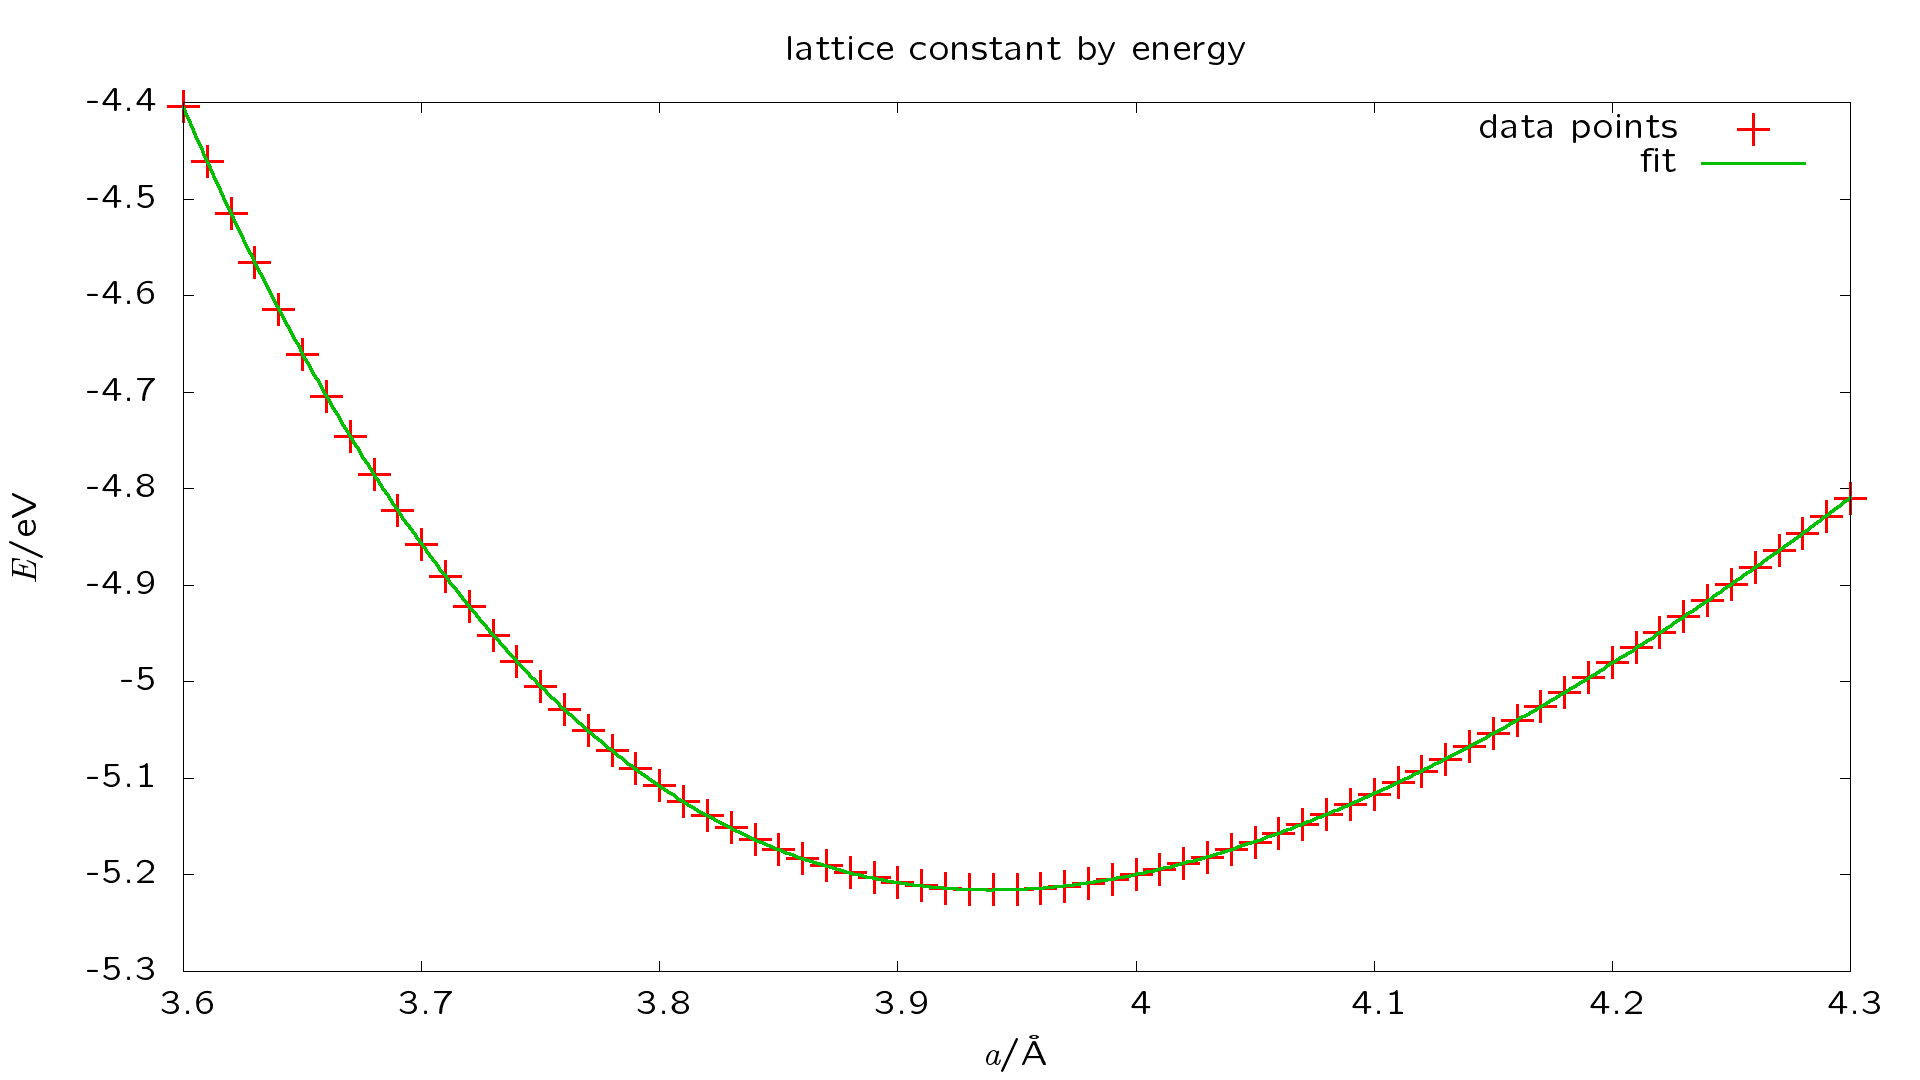
\includegraphics[width=0.7\textwidth]{Figures/BspFit.png}
\caption{An example of fitting different lattice constants with a polynomial expression. The optimal lattice constant is at the fit's minimum.}
\label{latfit}
\end{figure}
The guess with the lowest energy will be very close to the correct lattice-constant. If you fit a parabola through your energy-points, the minimum of the parabola will give the lattice constant (in case of Fig.\,\ref{latfit} that would be $a_0\approx3.96$). The goodness of the fit can be rated by eye inspection of a plot. A second order polynomial might not be a sufficient fitting function. In this case, use a fourth order polynomial. One needs to remember that such a polynomial has five fitting parameters, so one needs to make sure to use a much higher number of energy points to avoid overfitting. \\
\begin{figure}[h!!]
\begin{verbatim}
SYSTEM = Au: fcc
ENCUT = 300     
PREC = Normal   
LREAL = .False. 
SIGMA = 0.2
ISMEAR = 1              
GGA = 91       

NSW = 1     ! No ionic relaxation
     
IBRION = 1	 ! These parameters are
ISIF = 2    !   of no importance if no
POTIM = 0.5 !   ionic relaxation is performed.
\end{verbatim}
\caption{An exemplary INCAR-file for calculation of lattice constant via energy}
\label{bincar2}
\end{figure}

After the calculations for different ENCUTs and k-points (and whichever parameter was varied) are finished, the true lattice constant and the best set of parameters is chosen in the following manner:\\
\begin{figure}[h!!]
\centering
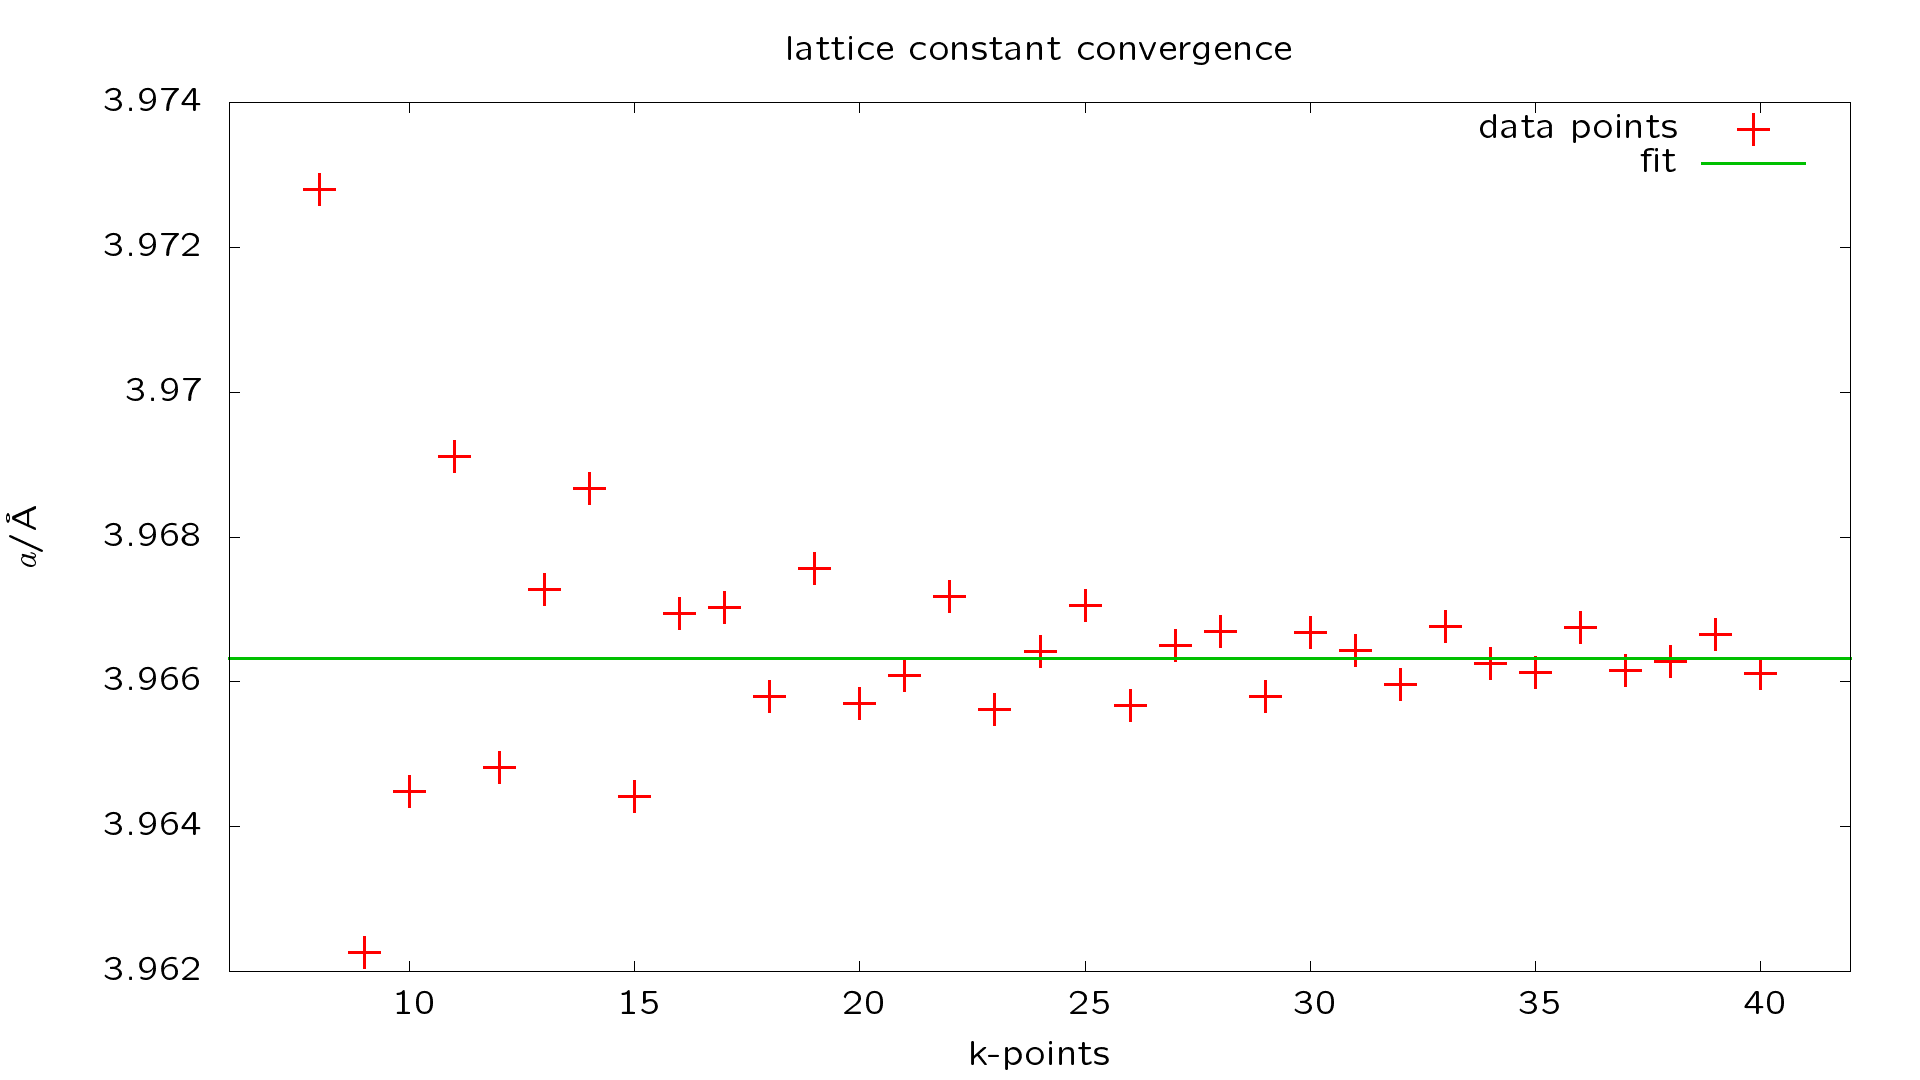
\includegraphics[width=0.7\textwidth]{Figures/SingleLatticeConstant.png}
\caption{Lattice constant convergence for different k-points.}
\label{kpfit}
\end{figure}
Plot the lattice constant for different k-points (cf Fig.\,\ref{kpfit}). For large k-points, the lattice constant should converge to a certain value ($a_0=3.9662$\,\AA~in case of Fig.\,\ref{kpfit}). This value should be regarded as the optimal value. Now, to get the best k-point set for further calculation, choose the lowest number of k-points that roughly (that is, within 0.001 eV or lower) reproduces your lattice constant (in case of Fig.\,\ref{kpfit}, that would be k-points 21 or 24). For the other VASP-parameters you varied, proceed accordingly.\\
Lastly, the SIGMA-parameter needs to be checked.\\
For that, vary the parameter SIGMA between 0.01 and 0.5. Once the calculations are done, the entropy needs to be determined. This can be done in two different way. You can check in the OUTCAR-file for the lowest occurrence of the line ``entropy T*S    EENTRO =" (cf. Fig.\,\ref{ent1}), or you can calculate the difference between the free energy and the energy without entropy. Both should be less than 1\,meV/atom. SIGMA should be as large as possible without compromising the energy of the system, so choose the largest SIGMA whose energy still corresponds to the energy of the calculations with lower SIGMA.\\
\begin{figure}[h!!]
\begin{verbatim}
 Free energy of the ion-electron system (eV)
  ---------------------------------------------------
  alpha Z        PSCENC =       116.98128788
  Ewald energy   TEWEN  =      -950.74055391
  -1/2 Hartree   DENC   =      -103.57651771
  -V(xc)+E(xc)   XCENC  =      -424.26980779
  PAW double counting   =          .00000000         .00000000
  entropy T*S    EENTRO =         -.00002139
  eigenvalues    EBANDS =         -.66210617
  atomic energy  EATOM  =      1360.63085531
  ---------------------------------------------------
  free energy    TOTEN  =        -1.63686377 eV

  energy without entropy =       -1.63684238  energy(sigma->0) =       -1.63685664  
\end{verbatim}
\caption{Finding the entropy in the OUTCAR-file.}
\label{ent1}
\end{figure}
\section{Slab-Calculations}
\label{slab}
Purpose:\\
The metal-slab terminates at the end of the surface to the vacuum. For the atoms of at least the surface layer, neighbours are missing. This can lead to a contraction or expansion of the interlayer distance of the first few layers of the slab. In theory, it can also lead to a reconstruction of the surface's geometry (cf e.g. herringbone reconstruction of Au(111)). Since the reconstruction usually takes place in larger unit cells than we can consider here, we omit reconstruction in $x$ and $y$-direction and only consider the interlayer-relaxation in $z$-direction.\\
For this, we fix the $x$ and $y$-coordinates of all atoms in the system and let the $z$-coordinate relax for all layers but the lowest two layers. The $z$-coordinates of the lowest two layers need to be fixed, too, to prevent the slab from drifting through space in $z$-direction and to give the above layers the impression that they are sitting on a metal-bulk.
\subsection{KPOINTS}
In the KPOINTS-file, a surface needs to be considered now by setting the last k-point to 1 (Fig.\,\ref{slabkp}).
\begin{figure}[h!!]
\begin{verbatim}
K-Points
0
Gammacentered
17 17 1
0 0 0
\end{verbatim}
\caption{Exemplary KPOINTS-file for the slab-relaxation.}
\label{slabkp}
\end{figure}
\subsection{POSCAR}
\begin{figure}[h!!]
\begin{verbatim}
  Au(111)  1 x 1  vac= 13.0000000000000000  A nlayer=  4
  1.000000
   2.970555537    .000000000    .000000000
  -1.485277768   2.572576696    .000000000
    .000000000    .000000000  20.276200000
   4
Selective dynamics
Cartesian
   .000000000   .000000000   .000000000  F  F  T
  1.485277813   .857525591 -2.425400000  F  F  T
   .000000000  1.715051182 -4.850800000  F  F  F
   .000000000   .000000000 -7.276200000  F  F  F
\end{verbatim}
\caption{Exemplary POSCAR-file for the slab-relaxation. Please note that the lattice constant has been multiplied into the cell-matrix and the coordinates and is therefore set to 1.0 in line 2.}
\label{spos}
\end{figure}
In the POSCAR-file, we now need to construct a slab. The first step for this is forcing periodic boundary conditions to see a slab of metal and not a bulk as before. We do that by enlarging the cell in $z$-direction and leaving part of the space without any atoms, that is, we create a vacuum of a certain thickness $vac$ above our slab. Because the periodic boundary conditions consequently do not replicate our single atom from the bulk-calculations in $z$-direction to form a continuous bulk, there is only one single layer of metal if only one atom is placed in the unit cell. If more layers are to be considered (which is advisable, since we want to model a slab and not only monolayer of the metal), more atoms need to be added into the unit cell, one for each layer (in $xy$-direction, the periodic boundary conditions still work perfectly fine). Another problem encountered is that, because we want to study a specific surface with its unique geometry, our cell matrix changes compared to the bulk (cf Fig.\,\ref{bposcar} vs Fig.\,\ref{spos}).\\
The cell-matrix consists of three lattice vectors written horizontally. Accordingly, line 3 of the POSCAR-file contains the lattice-vector in $x$-direction, line 4 the one in $y$-direction and line 5 the one in $z$-direction. For a (111)-surface, they can be calculated as follows:
\begin{equation}
c_x=a_0\left(\frac{1}{\sqrt{2}}, ~0.0, ~0.0\right)
\end{equation}
\begin{equation}
c_y=a_0\left(-\frac{1}{2\sqrt{2}}, ~\sqrt{\frac{3}{8}}, ~0.0\right)
\end{equation}
\begin{equation}
c_z= \left(0.0,~0.0,~\frac{(n_{lay}-1)a_0}{\sqrt{3}} + vac\right)
\end{equation}
Here, $a_0$ is the lattice constant from the bulk-calculations, $n_{lay}$ is the number of layers in the slab and $vac$ is the vacuum distance. It becomes evident why the lattice constant was multiplied into the cell matrix in the POSCAR-file in Fig.\,\ref{spos}; the $z$-coordinate of $c_z$ is not divisible by $a_0$ any longer. The complete cell matrix can looks as follows:
\begin{equation}
\begin{pmatrix}\begin{matrix} a_0 \frac{1}{\sqrt{2}} & 0.0 & 0.0 \\ a_0\frac{1}{2\sqrt{2}} & a_0 \sqrt{\frac{3}{8}} & 0.0 \\0.0 & 0.0 & \frac{(n_{lay}-1)a_0}{\sqrt{3}} + vac \end{matrix} \end{pmatrix}
\end{equation}
Furthermore, because we do not want to relax the entire cell now but only parts of the cell, we need to specify this in our POSCAR-file. This can be done by putting the command `selective dynamics' above the specification of the coordinate system. To tell VASP how to relax the coordinates, either T for `true' (relax) or F for `false' (keep fixed) need to be placed behind the coordinates of each atom, for each coordinate. Example: In line 9 of the POSCAR-file (cf Fig.\,\ref{spos}), the coordinates of the first atom are given. Because relaxation should only be done in $z$-direction, the $x$ and $y$-coordinates are fixed by writing F F at the end of the line. The $z$-coordinate is relaxed by placing T behind the two Fs.\\
A good first guess for $vac$ is $\approx 13$\,\AA. This should avoid interaction between the slabs created by the periodic boundary conditions.\\
In the exemplary POSCAR file in Fig.\,\ref{spos}, the $z$-coordinate $=0.0$\,\AA~is used to denote where the surface of the slab is.\\
\subsection{Convergence Tests}
First, the most advantageous parameters for the relaxation should be determined. For that, the following flags can (e.g.) be tested:\\
\textbf{ENCUT}: This flag does not necessarily need to be tested. The value obtained from the Bulk-calculations or the default should be fine.\\
\textbf{K-points}: The lowest number of k-points which still gives a converged result should be chosen. Check from 8 to $\sim$35.\\
\textbf{ISMEAR}: Dfferent smearing methods can but need not be tested. If not tested, ISMEAR = 1 is a good choice.\\
\textbf{Number of layers}: It might be useful to do the procedure for several layers while one is at it already.\\
$\textbf{vac}$: The thickness of the vacuum layer should be checked to avoid interactions between the slabs created by the periodic boundary conditions. (2-15\,\AA). The smaller the vacuum, the lower the calculation effort.\\
\textbf{EDIFF}: Different convergence criteria can be checked.\\
\textbf{SIGMA}: At the end of the convergence tests, SIGMA should be checked again. As mentioned in section\,\ref{bulk}, too large smearing values of SIGMA might lead to a wrong energy, but too low values require a larger kpoint-mesh. SIGMA should be as large as possible in order to minimise the difference between the free energy and the total energy.\\
\\
In the first step, the k-points need to be tested. For this, set IBRION = 1 or 2 and ISIF = 2 in the INCAR-file (cf Fig.\,\ref{slabincar1}) and test the k-points from 8 to $\sim$35. To avoid interaction of the slabs created through the periodical boundary conditions, set $vac$ to 13\,\AA in the POSCAR-file.
For each calculation, extract the `energy without entropy' from the OUTCAR-file after the calculations have finished and select the lowest k-points that reproduces the energy to which the larger k-points converge to. You can perform this procedure for several ISMEAR or check the behaviour of ISMEAR with the optimal k-point you get from the k-point-calculations here.
\begin{figure}[h!!]
\begin{verbatim}
System=Slab Au

PREC=Accurate
EDIFF=1E-05
EDIFFG=-1.0E-03

ISMEAR=1
SIGMA=0.1
ALGO=Fast

NSW=100
ISIF=2
IBRION=1
POTIM=0.6

GGA=RE
\end{verbatim}
\caption{Exemplary INCAR-file for the relaxation of the slab and the optimisation of the K-points and ISMEAR.}
\label{slabincar1}
\end{figure}
In the next step, evaluate the behaviour of the SIGMA. For this, set IBRION = -1 in the INCAR-file and remove the `Selective Dynamics' line and the corresponding `F' and `T' declarations form the POSCAR-file, or simply set $ \mathrm{NSW} = 1 $, invalidating IBRION by keeping the ions on fixed positions. Test SIGMA from 0.01 to $\sim$ 0.5. After the calculations, extract the value of the entropy from the OUTCAR-file either by looking for the bottommost occurrence of the line `entropy T*S    EENTRO =' or by calculating the difference between the free energy and the energy without entropy (cf Fig.\,\ref{ent1}). Choose SIGMA such that the value is maximal without compromising the energy, but less than 1\,meV/atom.\\
Once SIGMA is chosen, you can perform further tests for the thickness of the vacuum or the accuracy of the calculations (EDIFF). Make sure that no ionic relaxation is performed (I'm sure it'll also work if you have IBRION=1, ISIF=2 and $ \mathrm{NSW} > 1 $ and use the POSCAR from Fig.\,\ref{spos}, but it might take a little longer.)

\subsection{Relaxation of the slab}
For the relaxation of the slab, use the optimised results from the above section and put them into the INCAR and POSCAR-files given in Fig.\,\ref{slabincar1} and Fig.\,\ref{spos}. In the POSCAR-file, no matter how many layers you are considering, keep the lowest two layers fixed to give an impression of the bulk-interlayer distance.\\
Once the calculations are over, check whether the calculations have converged and if they have, extract the new interlayer distances from the CONTCAR-file. The calculations are converged if e.g. there is a line at the end of the OUTCAR-file saying `reached required accuracy - stopping structural energy minimisation' (Fig.\,\ref{sconv}).
\begin{figure}[h!!]
\begin{verbatim}
  FORCES: max atom, RMS      .000666     .000369
  FORCE total and by dimension     .000739     .000666


--------------------------------------------------------------------------------------------------------



 reached required accuracy - stopping structural energy minimisation
 writing wavefunctions
     LOOP+:  VPU time    1.07: CPU time    1.07


 General timing and accounting informations for this job:
 ========================================================

                  Total CPU time used (sec):       25.321
                            User time (sec):       24.972
                          System time (sec):         .349
                         Elapsed time (sec):       30.153

                   Maximum memory used (kb):      250432.
                   Average memory used (kb):           0.

                          Minor page faults:         4040
                          Major page faults:            2
                 Voluntary context switches:         2902                                                 
\end{verbatim}
\caption{Did the calculations converge?}
\label{sconv}
\end{figure}
If the calculation did not converge, consider raising the number of ionic (NSW) or electronic (NELM) steps or check for errors. The electronic energy needs to be converged to obtain accurate forces for the ionic relaxation.\\
In case you run into an error saying "ZBRENT: fatal error in bracketing please rerun with smaller EDIFF, or copy CONTCAR to POSCAR and continue", check if your EDIFF is reasonable, copy CONTCAR to POSCAR, set IBRION=1, ICHARG=1 and ISTART=1 in the INCAR file. Then you (re)start your calculation just as the one that produced the error. ICHARG and ISTART determine the type of calculation which is done. Setting them equal to one means to continue a previous calculation using the previously produces and nearly converged CHG, CHGCAR and WAVECAR files.\\
The CONTCAR file is a POSCAR-file that contains the result of the relaxation (cf Fig.\,\ref{contcar}). The positions are given in direct coordinates. You can transform them into Cartesian coordinates via applying the cell-matrix in a matrix transformation to the position and multiplying the resulting matrix by the lattice constant given in line 2.
\begin{figure}[h!!]
\begin{verbatim}
 1 x 1  vac= 13.000000000
 1.00000000000000000
     2.9705555370000001     .0000000000000000     .0000000000000000
    -1.4852777680000000    2.5725766960000001     .0000000000000000
      .0000000000000000     .0000000000000000   20.2761999999999993
   4
Selective dynamics
Direct
   .0000000000000000   .0000000000000000  -.0009317218716555   F   F   T
   .6666666865794397   .3333333433103576   .8787660531382623   F   F   T
   .3333333431981487   .6666666866207223   .7607638512147261   F   F   F
   .0000000000000000   .0000000000000000   .6411457768220856   F   F   F

   .00000000E+00   .00000000E+00   .00000000E+00
   .00000000E+00   .00000000E+00   .00000000E+00
   .00000000E+00   .00000000E+00   .00000000E+00
   .00000000E+00   .00000000E+00   .00000000E+00

\end{verbatim}
\caption{The CONTCAR-file contains the new positions after the relaxation, but in direct coordinates.}
\label{contcar}
\end{figure}
Either use the CONTCAR-file as a POSCAR-file for the next calculations or extract the interlayer distance and form a new POSCAR-file to continue.

\section{Convergence tests on Surface + H calculations}
\label{H+slab}
For the convergence test, the difference in energy between an H-atom 6.0\,\AA~above the slab's surface and on the slab's surface (1.1\,\AA) is tested. \\
The \textbf{KPOINTS-file} stays the same as for the slab-calculations, with the set of k-points deemed optimal during the convergence test for the slab-calculations. 
The \textbf{POTCAR-file} for the metal needs to be unified with a POTCAR-file for H.
\subsection{The POSCAR-file}
Use the new POSCAR-file with the relaxed interlayer distance from Section\,\ref{slab}. Remove everything from the POSCAR that refers to relaxations, that is, the line `selective dynamics' and the Fs and Ts at the end of the single Au-atom coordinates.\\
New about the POSCAR-file in this step of the calculations is that a hydrogen atom is added to the calculation. That changes two things. For one, the cell-size needs to be increased to avoid interaction between the hydrogen atom with its images created from the periodic boundary conditions. So far, the POSCAR-file had a $1\times1\times n_{lay}$-cell where $n_{lay}$ is the number of layers in the cell. Now, the cell-size is increased by one atom in each $x$- and $y$-direction and a $2\times2\times n_{lay}$ is formed (cf Fig.\,\ref{cpos}). Larger cell-sizes are imaginable, but for the creation of the potential energy surface (PES), AIMD trajectories will later need to be produced which are computationally very demanding, and larger cell-sizes will add a considerable number of atoms which will increase the computational effort tremendously.\\
Furthermore, the H-atom needs to be added to the POSCAR-file. This is done by adding the number of H-atoms in the cell (1) to line 6. Because the H-atom is an atom of a different species than the Au-atoms, its number is not added to the number of metal-atoms (24, cf Fig.\,\ref{cpos}) but written behind the number of metal atoms. The ordering here needs to be the same as in the POTCAR-file. That is, if the metal-POTCAR-file comes first and the H-POTCAR-file was added behind it, in the POSCAR-file the number and positions of the metal-atoms must come first and the H-number and position after that. Therefore, in our case, the position of the H-atom is written below the positions of the metal atoms.
\begin{figure}[h!!]
\begin{verbatim}
  H + Au(111)  2 x 2  vac= 13.0000000000000000  A nlayer=  6 
  1.000000
   5.941111074    .000000000    .000000000
  -2.970555537   5.145153392    .000000000
    .000000000    .000000000  25.107500000
  24   1
Cartesian
    .000000000    .000000000    .000000000
   2.970555537    .000000000    .000000000
  -1.485277768   2.572576696    .000000000
   1.485277768   2.572576696    .000000000
   1.485277813    .857525591  -2.451700000
   4.455833350    .857525591  -2.451700000
    .000000044   3.430102287  -2.451700000
   2.970555581   3.430102287  -2.451700000
    .000000000   1.715051182  -4.857500000
   2.970555537   1.715051182  -4.857500000
  -1.485277768   4.287627878  -4.857500000
   1.485277768   4.287627878  -4.857500000
    .000000000    .000000000  -7.254500000
   2.970555537    .000000000  -7.254500000
  -1.485277768   2.572576696  -7.254500000
   1.485277768   2.572576696  -7.254500000
   1.485277813    .857525591  -9.682100000
   4.455833350    .857525591  -9.682100000
    .000000044   3.430102287  -9.682100000
   2.970555581   3.430102287  -9.682100000
    .000000000   1.715051182 -12.107500000
   2.970555537   1.715051182 -12.107500000
  -1.485277768   4.287627878 -12.107500000
   1.485277768   4.287627878 -12.107500000
    .000000000   1.715051182   6.000000000

\end{verbatim}
\caption{Exemplary POSCAR-file. H-atom was placed above the fcc-hollow site.}
\label{cpos}
\end{figure}
\clearpage
Two POSCAR-files need to be produced for this step of the calculations. One where the H-atom is 6.0\,\AA~above the surface and one where the H-atom is close to the surface ($\sim 1.1$\,\AA). For the $x$- and $y$-coordinate of the system, one of the recognisable surface sites is advisable like top, bridge or one of the two hollow sites.\\
\subsection{The INCAR-file}
\begin{figure}[h!!]
\begin{verbatim}
   ALGO=F
   NELM = 120
   GGA = RP
   ISYM = 1
   ISPIN = 2			! Calculate the spin
   LWAVE = .FALSE.		! Don't print the WAVECAR, they waste memory space here
   LCHARG = .FALSE.		! Don't print the CHG-files, they waste memory space here
   AMIX = 0.3			! These settings are good.
   BMIX = 0.0001		!
   AMIX_MAG = 0.3		!
   BMIX_MAG = 0.0001	!
   MAXMIX = 20			!

   PREC = Accurate
   SIGMA = 0.1
   ISMEAR = -1
   EDIFF = 1.0E-4

   MAGMOM = 25*1.0
   ENMAX  = 350			! Another way to specify ENCUT
\end{verbatim}
\caption{Exemplary INCAR-file. Note the magnetic moment (MAGMOM) and the spin (ISPIN) that is now specified.}
\label{cin}
\end{figure}
The H-atom has a free electron, therefore, it has a spin and a magnetic moment. This needs to be accounted for. At the end of the optimisation, you can check if it makes a difference to specify it or not.\\
I have been told that ISMEAR = -1 is the best setting for ISMEAR you can choose for H+metal. You are welcome to check it. But remember, you must not continue any calculations with ISMEAR = -1 that have been performed earlier with another value of ISMEAR. That is, if you did your slab relaxation with ISMEAR = 1, you must not select ISMEAR = -1 for your H@Metal-system.\\
\subsection{Convergence tests}
Again, the number of \textbf{K-points} should be checked (8-35).\\
\textbf{ENCUT}: Start with the highest of the specified ENMAX-tag of both concatenated POTCAR files. Increase it in steps of 50 eV until convergence is accomplished. If no convergence can be observed, give it the value of the highest ENMAX.\\
\textbf{Number of layers}: Either choose the number of layers you would like to have to fit your PES or check which number of layers with which number of k-points, ENCUT and SIGMA calculates fastest while still giving the same result as the most expensive calculations.\\
\textbf{SIGMA}: For sigma, proceed as described in the sections above. Check how thick your \textbf{Vacuum-layer} needs to be. Again, 13\,\AA seems a good guess to begin with.\\
Again, start out with checking which number of k-points you need. For that, set ENCUT to its default-value, SIGMA to the value from the slab-calculations and the vacuum distance to 13\,\AA.\\
Of course, check also whatever other parameter you want.\\
If you want to be very thorough, test the dependence of each of these parameters from each other. That is: calculate the k-point- and ENCUT- and SIGMA-dependence for every change in the vacuum distance you consider and vice versa.\\
In general, choose your parameters in such a way that they still reproduce the energy-difference for the most accurate calculations (that is: those calculations that have the highest number of k-points, highest ENCUT and largest vacuum layer). For the energy-difference, get the `energy sigma $\rightarrow 0$: ' from the OUTCAR-file (cf Fig.\,\ref{boutcar1}) for both positions of the hydrogen atom and subtract the energy of H at 6.0\,\AA~from the energy of H at 1.1\,\AA.
By the end of this optimisation, you should have your perfect parameters to start building up your PES.\\
\subsection{Spin restricted or Spin unrestricted calculations?}
VASP offers the possibility to calculate the energy of the hydrogen atom with and without involving the spin. As long as the hydrogen atom is close to the surface, the spin should not play any role, for the interaction with the Au's atoms should even out the spin. When the H-atom is far away from the surface, though, the spin becomes important.\\
The parameter in VASP that governs if the spin is calculated or not is \textbf{ISPIN}. For ISPIN=1, the calculations are performed non-spin-polarized and for ISPIN = 2, spin-polarized calculations are being performed. If the second option is chosen, the flag \textbf{MAGMOM} can also be specified. If you count the number of ions $N$ you have in your POSCAR-file and set MAGMOM= $N*1.0$, you should be fine.\\
Finally, do another calculation with the H-atom above and at the surface with and without magnetic moment and spin. If the energy is not different, neglect the magnetic moment for the ongoing calculations.\\
It is more likely that you will need to take the spin into account. If you are not restricted on calculation time, take the spin into account for your entire energy grid.


\section{The Potential Energy Surface}
\subsection{The H-atom-grid}
An exemplary INCAR-file for these calculations is shown in Fig.\,\ref{cin}.
The first step consists of building an energy-configuration grid in which metal-atoms are at their previously calculated relaxed surface layer positions and the H-atom is moved on a narrow grid to sample the configuration space. So far, we have taken a grid of ten sites on the metals surface that focuses on surface sites with distinct symmetrical properties (cf Fig.\,\ref{surfacesites}).
\begin{figure}[t!]
\centering
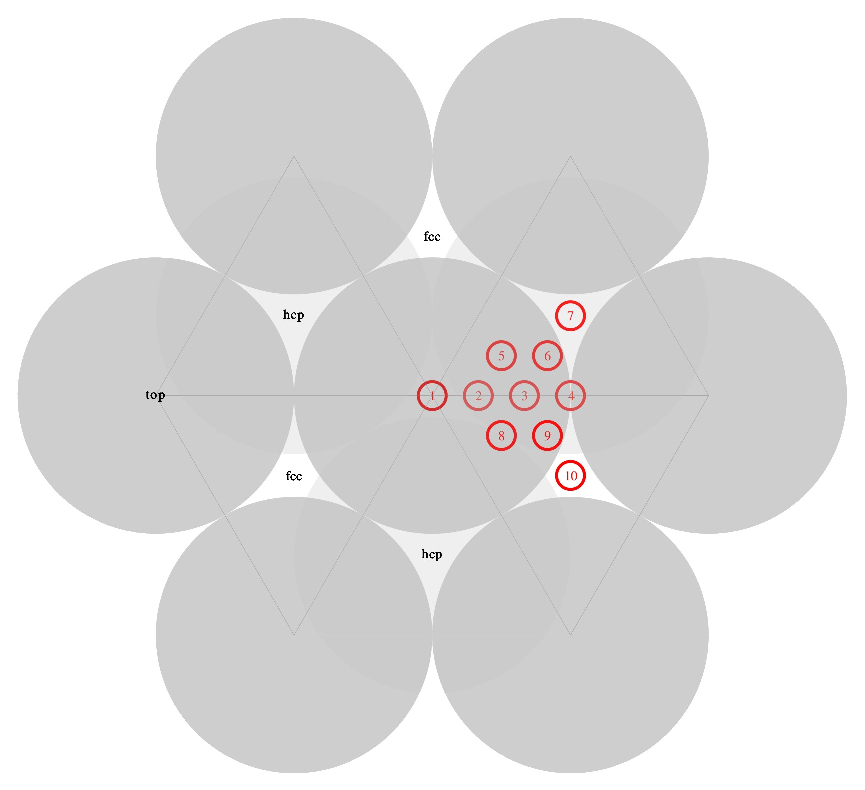
\includegraphics[width=0.7\textwidth]{Figures/SurfaceSites}
\caption{Ten Surface Sites for the PES.}
\label{surfacesites}
\end{figure}
The points 1 to 4 scan the region from the top site (1) to the bridge site (4). (1)-(5)-(7) maps out the straight line from the top site to the hcp-hollow site (7) and (1)-(8)-(10) from the top site to the fcc-hollow site (10). (6) and (9) sample the site of the metal atom. The H-atom should be moved perpendicular (that is, keeping the $x$- and $y$-coordinates fixed) to each of these sites starting from 6\,\AA~above the surface to the bottom layer of the slab in steps of 0.2\,\AA. The $x$- and $y$-coordinates of the points can be calculated as shown in Tab.\,\ref{calsusi}.
\begin{table}[h!]
\centering
\caption{How to calculate the $x$- and $y$-positions of the ten surface sites.}
\label{calsusi}
\begin{tabular}{ccc}
\hline\hline
Site&$x$-coordinate&$y$-coordinate\\
\hline
1&0.0						&0.0\\
2& $\frac{a_0}{6\sqrt{2}}$	&0.0\\
3& $\frac{a_0}{3\sqrt{2}}$	&0.0\\
4& $\frac{a_0}{\sqrt{8}}$	&0.0\\
5& $\frac{a_0}{4 \sqrt{2}}$	&$\frac{\sqrt{3}}{12\sqrt{2}}a_0$\\
6& $\frac{5}{12\sqrt{2}}a_0$&$\frac{\sqrt{3}}{12\sqrt{2}}a_0$\\
7& $\frac{a_0}{\sqrt{8}}$	&$\frac{\sqrt{3}}{6\sqrt{2}}a_0$\\
8& $\frac{a_0}{4\sqrt{2}}$	&$-\frac{\sqrt{3}}{12\sqrt{2}}a_0$\\
9& $\frac{5}{12\sqrt{2}}a_0$&$-\frac{\sqrt{3}}{12\sqrt{2}}a_0$\\
10&$\frac{a_0}{\sqrt{8}}$ 	&$-\frac{\sqrt{3}}{6\sqrt{2}}a_0$\\
\hline\hline
\end{tabular}
\end{table}\newline\noindent
Extract from the OUTCAR-files of each calculation the `energy sigma $\rightarrow$ 0' -energy. The energy when the H-atom is above the fcc-site and 6.0\,\AA~above the surface serves also as \textbf{reference energy}.
\subsection{The AIMD-trajectories}
Part of the fitting procedure also includes taking geometries at which the metal-atoms are not on their equilibrium positions and the H-atom is on other plausible positions that it might take up during a trajectory. To sample that configuration space, we take geometries from an AIMD-trajectory calculated for the very same system. Because we have not yet found out what kind of AIMD-geometries might give the best contribution to a fit, it is best to calculate roughly 20 AIMD-trajectories and use geometries from each of these trajectories as input for the fit.\\
I have no idea how to actually calculate AIMD trajectories, but I hope someone else can oblige here.

\section{Fitting the Potential Energy Surface with EMT}
\subsection{The parameters}
The Effective Medium Theory developed by N\o rskov \emph{et al.}\,\cite{jacobsen1996,jacobsen1987} has seven parameters per species which are related to the physical properties of the species.\\
There are $\eta_2$, $n_0$, $E_0$, $\lambda$, $V_0$, $\kappa$ and $s_0$.
$s_0$ is the neutral sphere radius. It is calculated (Eq.\,) as follows from the lattice constant $a_0$ determined in the bulk-calculations:
\begin{equation}
s_0 = \frac{a_0}{\beta' \sqrt{2}}
\end{equation}
Here, $\beta'$ is a geometrical factor for the fcc-crystal:
\begin{equation}
\beta' = \frac{\sqrt[3]{16 \pi /3}}{\sqrt{2}}
\end{equation}
$E_0$ is the cohesive energy (sublimation energy) which can be found in literature. 
Together with $\lambda$, $E_0$ and $s_0$ are directly related to the bulk modulus:\\
\begin{equation}
B = -\frac{E_0 \lambda^2}{12 \pi s_0}
\end{equation}
$s_0$ is furthermore related to the shear modulus, together with $\kappa$, $\eta_2$ and $V_0$:\\
\begin{equation}
C_{44} = \frac{3 V_0 \kappa \delta}{8\pi s_0}
\label{c44}
\end{equation}
As well as the other elastic constants:
\begin{equation}
C_{11}=\frac{3 V_0 \delta \kappa -E_0 \lambda^2}{12 \pi s_0}
\end{equation}
\begin{equation}
C_{12}=\frac{3 V_0(\kappa-\beta'\eta_2)\kappa-2E_0\lambda^2}{24\pi s_0}
\end{equation}
with 
\begin{equation}
\delta = \beta'\eta_2-\kappa
\end{equation}
$n_0$ is a parameter relating to the individual density of the species and responsible for the coupling between species.\\
\subsubsection*{Recommendations for the parameters}
\textbf{Parameters for the metal} (Me)\\
All the parameters apart for $E_{0,Me}$ should have positive values.
$s_{0,Me}$ and $E_{0,Me}$ should be kept constant during the fit to reproduce the most important bulk properties. If you varied $s_{0,Me}$, you would also change the lattice constant of your metal and that does not make very much sense since you spent a lot of time actually finding the right one. Varying $E_{0,Me}$ will mostly destabilise the fit anyway, but it will also lead to PES which melt at very low temperatures (if $E_{0,Me}$ is too small) or not at all. So, it's not advisable to change this parameter. $\lambda_{Me}$ is a parameter you can keep fixed during the fitting procedure so the experimental bulk-modulus is reproduced. Actually fitting it might improve the fit slightly, but then, you won't reproduce the bulk-modulus as accurately anymore.\\
Furthermore, you should keep $\kappa_{Me}$, $\eta_{2,Me}$ and $V_{0,Me}$ such that they roughly reproduce the shear-modulus. For Au, $C_{44}$ (without $s$) should be $C_{44} \ge 10^{10}$ and best $C_{44} \ge 1.2 \cdot 10^{10}$. The melting temperature of the slab is in some obscure way related to $C_{44}$. I haven't figured out in which way, yet, but if your shear modulus gets too small (smaller than the numbers I recommend here), the surface will start disintegrating at unreasonably low temperatures.\\
As far as I've seen it, there aren't any issues related to $n_{0,Me}$..\\
\begin{table}[h!]
\centering
\caption{Recommendations for the metal parameters.}
\label{calsusi}
\begin{tabular}{ccc}
\hline\hline
Parameter&Relation to metal properties&Recommendation\\
\hline
$s_0$& $s_0= \frac{a_0}{\beta' \sqrt{2}}$& fix\\
$E_0$& Cohesive/Sublimation Energy& fix\\
$\lambda$&$B = -\frac{E_0 \lambda^2}{12 \pi s_0}$& (fix)\\
$\eta_2$, $\kappa$, $V_0$&$C_{44} = \frac{s\cdot V_0\cdot \kappa (\beta'\eta_2-\kappa)}{8\pi s_0}$& restrain\\
$n_0$& density& none\\
\hline\hline
\end{tabular}
\end{table}
\textbf{Parameters for Hydrogen}\\
There is no experimental data for metallic hydrogen that I know of. I therefore recommend to use the values suggested by Strömquist \emph{et al}\,\cite{strom1998} as a first guess but try to vary all of them during the calculations.\\
In general, you should not fit all hydrogen parameters at once, because that will destabilise the fit; if you are fitting $s_{0,H}$, $E_{0,H}$ should not fitted simultaneously and vice versa. The values suggested by Strömquist \emph{et al} for $s_{0,H}$ and $E_{0,H}$ result in good fits, so you do not necessarily need to fit them. If you decide to do so, for fitting $s_{0,H}$, I would recommend to set a guess-$s_{0,H}$ before you start the actual fitting. The estimated lattice constant for metallic hydrogen is around 0.88\,\AA~resulting in $s_{0,H}=0.49$\,\AA\,\cite{wigner1935}, you should take note, though, that lowering $s_{0,H}$ also reduces the density the H-atom feels. In the nonadiabatic calculations, this would decrease the friction coefficient.\\
If you are fitting $s_{0,H}$ or $E_{0,H}$, I would first fit them with some of the other parameters and after that perform another fit in which you take the new values for $s_{0,H}$ or $E_{0,H}$ from your previous fit, but optimise the other parameters separately.\\
\begin{figure}[t!]
\begin{verbatim}
   eta2=             5.4254d0
     n0=             0.182205d0
     E0=            -2.37100000
 lambda=             7.72709d0
     V0=             0.427d0
  kappa=             8.86282d0
     s0=             0.68041100
\end{verbatim}
\caption{Exemplary file for the H-parameters. File contains the values suggested by Strömquist \emph{et al}. Please don't change the order of the parameters.}
\label{Mdtianfit}
\end{figure}
\subsection{Performing the fit}
\begin{figure}[t!]
\begin{verbatim}
projectile H 1.0079 7 'fitdata/emt573_H.nml' ver 0
lattice Au 196.96657 7 'fitdata/emt573_Au.nml' ver 0
pes emt
celldim 2 2 4 x
rep 1 1
conf fit au111_2x2x4.POSCAR 10 987
aimd 700 200 0.00
evasp -24.995689d0  ! A value for Au 2x2
fitconst 14 1 2 3 4 5 6 7 8 9 10 11 12 13 14
maxit 1
\end{verbatim}
\caption{Exemplary input-file for the fit in the MD\_tian Programm.}
\label{Mdtianfit}
\end{figure}
The input-file (cf Fig.\,\ref{Mdtianfit}) for the fit begins with the specification of the two species fitted. `projectile' classifies the projectile, in our case, the hydrogen atom. `lattice' specifies the metal slab. The flag is followed by the name of the projectile, its mass, the number of parameters, the file-name of the file that contains the starting parameters, the algorithm and the number of layers that should be kept fixed for eventual MD-simulations. The last two variables can be safely ignored for fitting. Next, `pes' declares for which theory the PES should be fitted. `celldim' records the dimensions of your input-cell as described for the optimisation of the H/Metal-system. `rep' organises how many times your cell should be replicated to produce a cell that is fit for EMT-usage. `rep 1 1' is a reasonable choice. 
`conf' determines if the program is going to be doing MD-simulations or fitting. For fitting, `conf' should be followed by `fit', the name of the POSCAR-file that contains your equilibrium structure with the H-atoms 6.0\,\AA~above the surface, the number of the AIMD-trajectory you would like to fit (in this case 10) and the number of the fit (in this case 987).\\
`aimd' controls the AIMD-contribution. The flag is followed by the number of Equilibrium-DFT-Points you would like to use, then by the number of AIMD-DFT-points and finally by de\_aimd\_max which determines how the AIMD-points should be chosen. If it is set to 0.0, then the points will be chosen in regular intervals from the trajectory. For larger values, a point is only then used in fitting if its energy-difference to the preceding point is larger than de\_aimd\_max.\\
`evasp' controls the reference energy. It is followed by the energy a hydrogen atom has at 6.0\,\AA~above an equilibrated Au-surface (see previous section for determination of the reference energy).\\
`fitconst' determines which parameters should be kept fixed. Thus, the integer behind it is the number of fixed parameters in the fit, followed by the numbers corresponding to the fixed parameter. The numbers are assigned as follows (Tab.\,\ref{nopar}).\\
\begin{table}[t!]
\centering
\caption{Number of parameter for fitting.}
\label{nopar}
\begin{tabular}{rrrr}
\hline\hline
No.&Parameter&No.&Parameter\\
\hline
1&$\eta_{2,H}$	&8&$\eta_{0,metal}$\\
2&$n_{0,H}$		&9&$n_{0,metal}$\\
3&$E_{0,H}$		&10&$E_{0,metal}$\\
4&$\lambda_{H}$	&11&$\lambda_{metal}$\\
5&$V_{0,H}$		&13&$V_{0,metal}$\\
6&$\kappa_{H}$	&12&$\kappa_{metal}$\\
7&$s_{0,H}$		&14&$s_{0,metal}$\\
\hline\hline
\end{tabular}
\end{table}
`maxit' Maximal number of iteration. Followed by the maximal number of iterations. 100 is a good choice here.\\
\subsubsection*{Recommendations for the fitting}
Use a ratio of 5:2 between your Equilibrium- and AIMD-DFT Points. This appears to give good results. But we should do more detailed testing here.\\
Some AIMD-trajectories will work better for the fit than others. In my experience, trajectories in which the hydrogen atom spends a long time in the subsurface are not quite as suited as single- or double bounce trajectories. In our fitting procedure, you can decide between either taking regularly spaced points from the AIMD-trajectory (de\_aimd\_max = 0.0) or only such points that differ by a certain energy from the previous point (de\_aimd\_max = x). In my experience, taking equally spaced points works better. Also, you can decide points up to a certain energy should be taken into account (e\_max). In the program, this value is set to 20\,eV which I found to be suited best.
\subsection{After the Fit}
After the fit, the physically reasonable behaviour of the fit and its convergence needs to be determined. To check the convergence, calculate the rms to the input-data and the rms to the remaining AIMD-trajectories. If those values are both below 190\,meV, the fit can be considered a candidate.

\subsubsection*{Checking the Physical Behaviour of the Fit}
The first check is calculating $C_{44}$ (cf Eq.\,\ref{c44}). If the fit's $C_{44}\ll s\cdot1.2\cdot10^{10}$ the metal-surface will probably disintegrate at a too low temperature. You can test this by running MD-trajectories for different temperatures which propagate the motion for the metal-surface for several pico-seconds and by checking if the metal-slab still retains its shape as a surface after the trajectories.\\
Furthermore, you should also check if the H-atom can abstract metal-atoms from the surface. For that, you calculate the energy an H-atom has at 6\,\AA~above the surface. Then do the same calculations, only additionally to the H-atom at 6\,\AA, remove a metal-atom from the surface and place it at the distance of the H-metal-bond above the H-atom. With that I mean: Form a vacancy in the surface and use the atom from this vacancy to create a metal-H-molecule that is also 6\,\AA~above the surface.\\
Calculate from the difference the energy $\zeta$ that is needed to form an H-metal molecule from a surface atom and an H-atom. We should probably implement a subroutine into the fitting procedure that does that automatically at the end of the fit.\\
\begin{equation}
\zeta = \Delta_\mathrm{f} H^\circ(\mathrm{Au_{s\rightarrow g}})-\Delta_\mathrm{f}H^\circ(\mathrm{Au-H})
\label{zeta}
\end{equation}
Compare the value to experimental values. $\zeta$ can be calculated by subtracting the metal-H-formation energy from the sublimation energy of the metal (cf Eq.\,\ref{zeta}). The value obtained for your fit should not be much below it.
\begin{table}[t!]
\centering
\caption{The arts of metal-H formation.}
\label{auh}
\begin{tabular}{ccccc}
\hline\hline
Metal&$\Delta_\mathrm{f} H^\circ(\mathrm{Au_{s\rightarrow g}})$(eV)&$\Delta_\mathrm{f}H^\circ(\mathrm{Au-H})$(eV)&bond length (\AA)&$\zeta$ (eV)\\
\hline
Au&3.8\cite{hildenbrand1962}&2.99\,\cite{kant1979}&1.52 (CRC)&0.8\\
Cu&&2.53\,\cite{kant1979}&&\\
Ag&&2.19\,\cite{kant1979}&&\\
Ni&&2.58\,\cite{kant1979}&&\\
\hline\hline
\end{tabular}
\end{table}

\subsection{Possible issues}
If the fit has problems converging, you can first try fitting to the equilibrium-GGA-DFT-points and use the resulting parameters as input in a new fit where you then include both the equilibrium-DFT-points and the aimd-DFT-points.
Last but not least: form a circle of salt around your computer before starting the fitting and sacrifice a few drops of water to Thoth.\\

\chapter{Skycruizer}

\chapter{Function of the single modules and subroutines}
\section{atom\_class}
\index{atom\_class}
This model contains all parameters that cannot be changed during the execution of the program as well as some default values. This includes commonly used irrational numbers and physical constants and unit-conversion factors. Furthermore, the object atoms and its allocation defined which holds information such as the positions, velocities, forces \&c about the particle or the lattice.

Also, the program's basic units \index{units} \index{program basic units} are defined. They are:\\
Length: \AA\\
Time: fs\\
Energy: \\
The program-derived units\index{program derived units} are:\\
Mass: eV$\cdot$fs$^2$/\AA$^2$ = $1/103.6382$\,amu\\
Angle: radian = 180$^\circ$\\
bohr: 0.5291772\,\AA
\section{dtrnlspbc}
\index{dtrnlspbc}
\todo{describe}
\section{fit4tian}
\index{fit4tian}
This is the interface for the fitting routine. It contains the following subroutines:
\textbf{fit}\\
Here, the fit is prepared. The parameter files and the input into the fit are formed and information on the beginning and end of the fit are printed out. The non-linear least square algorithm with boundary constraints is prepared and called.
 
\textbf{dev2eqdft}\\
Generates the dev2Eqdt$n$.dat output file of the fit. This file relates to the 3D-grid and for a fixed surface samples the ten surface sites starting from 6\,\AA~above the surface with whatever step and to whatever depth is defined in the Eq\_points\_dft.dat-file. Each position is followed by the potential energy calculated with the fit's parameter set at surface atoms frozen to their relaxed position for that position of the particle.
\textbf{denseqdf}\\
This routine is almost identical to the above, only instead of the potential energy, the denseqdft$n$.dat-file contains the background electron density at these positions.
\textbf{dev2aimddft}\\
\label{Sec:Function:f4t:dev2aimd}
This routine produces the traj$n$\_1.dat file. This file is related to the AIMD-trajectories that are used in the input-data set and control data set for the fit. It contains the step of each trajectory followed by the potential energy from the DFT-simulations and then by the potential energy calculated with the fit parameters from the positions corresponding to the step.

Furthermore, information on the fit (number, shear modulus, the H-metal bond formation energy, rms-error to the testing set (it consisting of all the AIMD-trajectories) and the parameter values) are printed into the c44rms.dat-file and information on the fit (rms-error to the testing set, elastic moduli) are printed out.

\textbf{readinaimd}\\
This routine is called up by the dev2aimddft-routine (see Sec.\,\ref{Sec:Function:f4t:dev2aimd}) and reads in the positions and energies of the XDATCAR.dat and analyse.dat files, respectively, of the AIMD trajectories. It proceeds to produce a $6\times6$ surface cell from the data so the EMT-routine can be used to calculate the energy from the AIMD positions.

\textbf{restricted\_fit}\\
\todo{restricted\_fit}

\section{Force}
\index{force}
This module deals with the calculation of energies, forces and analytic derivatives of the PES usable in the program as well as the routine that calculates the friction coefficient from the local density. In general, the subroutines fall into three classes. The ones with a `1' at the end of the name deal with the calculation of only one species. Those with `\_e' at the end calculate only the energy without the forces and the ones with `d' (e.g. de or ddens) also includes routines to calculate the derivatives with respect to the parameters (see Tab.\,\ref{Tab:Funct:force}).

\begin{table}[b!]
\centering
\caption{Subroutines in the force-module and what they calculate (BED = background electron density\index{BED}).\\
$^{(1)}$ only next neighbors included.\\
$^{(2)}$ calculated numerically.\\
$^{(3)}$ calculates the friction coefficient from the BED.}
\label{Tab:Funct:force}
\begin{tabular}{lllllll}
\hline\hline
name			&No.	& energy	&forces			&BED		&parameter	& system\\
&species&&&&derivatives&\\
\hline
emt				&2				&$\times$	&$\times$		&$\times$	&						&EMT\\
emt\_e 			&2 				&$\times$	&				&$\times$	&						&EMT\\
emt1			&1				&$\times$	&$\times$		&$\times$	&						&EMT\\
emt1\_e 		&1				&$\times$	&				&$\times$	&						&EMT\\
emt\_e\_fit 	&2 				&$\times$	&				&			&						&EMT\\
emt\_de\_fit 	&2				&$\times$	&				&$\times$	&$\times$ (to energy)	&EMT\\
emt\_dens\_fit	&2				&$\times$	&				&$\times$	&						&EMT\\
emt\_ddens\_fit	&2				&$\times$	&				&$\times$	&$\times$ (to density)	&EMT\\
emt1nn			&2				&$\times$	&$\times$		&$\times$	&						&EMT$^{(1)}$\\
num\_emt		&2				&$\times$	&$\times^{(2)}$	&$\times$	&						&EMT\\
num\_emt1		&1				&$\times$	&$\times^{(2)}$	&$\times$	&						&EMT\\
ldfa			&1				&			&				&			&						&LDFA$^{(3)}$\\
lj\_e			&2				&$\times$	&				&			&						&Lennard-Jones\\
lj				&2				&$\times$	&$\times$		&			&						&Lennard-Jones\\
lj1\_e			&1				&$\times$	&				&			&						&Lennard-Jones\\
lj1				&1				&$\times$	&$\times$		&			&						&Lennard-Jones\\

\hline
\hline
\end{tabular}
\end{table}

In the LDFA subroutine, the friction coefficient is calculated from the local background electron density. The variable containing the local background electron density is then overwritten by the friction coefficient (in fs$^{-1}$). In case of simulated annealing a general friction coefficient of 3\,ps$^{-1}$ is assumed.

\section{md\_init}
\index{md\_init}
This module is a monster. Tab.\,\ref{Tab:Funct:mdinit} gives an overview over the subroutines in the module and their purpose. In general, this module serves as an initialization module for (almost) everything that goes into the program. Due to this reason, it starts with a large block of global variable that need to be used in other modules as well.
\begin{table}[b!]
\centering
\caption{Subroutines in the md\_init module and their purpse.}
\label{Tab:Funct:mdinit}
\begin{tabular}{ll}
\hline\hline
name			&purpose			\\
\hline
simbox\_init & read input file, calls up dependent on \textit{confname}\\
read\_conf&\\
prep\_slab&\\
prep\_teil&\\
read\_mxt&\\
read\_fit&\\
traj\_init&\\
particle\_init&\\

\hline
\hline
\end{tabular}
\end{table}

\section{md\_tian}
\index{md\_tian}
This is the main program-file that calls up all other routines. It starts with calling the simbox\_init-routine to initiate the program and then calculates the reference energy. According to \textit{confname}, either fit or MD-routine are started. The first is started by calling up \textbf{fit4tian}, in the second case, the loop over the trajectories starts in the main program with initiating the species, followed by a loop over the time steps that calls up the propagators in \textbf{mdalgo} for the propagation of the trajectory. The routines for the output are also called here. Furthermore, the collectors for the number of bounces\index{bounces}, the collector (pEfric) for the energy loss to phonons (when md\_algo\_p = 3 or 4 (Langevin dynamics)) or to calculate electronic friction post facto (pEF, when md\_algo\_p = 5 (Verlet with pEF)), the collector for the lowest particle position and the routine that stops a trajectory when the particle has moved through the slab or scattered further back than 6.1\,\AA from the surface are to be found here.

MD-simulations are either the calculation of trajectories or simulated annealing. The decision between the former and latter is controlled by the variable \textit{sasteps} that also controls when the surface temperature during the simulated annealing is to be lowered or raised.

The number of bounces is calculated by finding maxima in the background electron density. The reasoning behind this is that if a particle gets close to a surface atom, the electron density must rise; it will peak when the particle is closest to the surface atom. To avoid double-counting of maxima due to fluctuations in the BED, a bounce is only counted if the minimum between two maxima is larger than 0.025\,\AA$^{-3}$. This is not a perfect way to count the number of bounces, but the best we could come up with so far.

At the end, there are some lines commented out that make it possible to calculate the timing  of the program if they are commented in again.

\section{mdalgo}
\index{mdalgo}
This routine contains the propagation algorithms divided into their first (propagator\_1) and second step (propagator\_2). Those algorithms are: the Verlet Algorithm\,\cite{allen1989}, the Beeman-Refson Algorithm\,\cite{refson1985}, the Langevin algorithm\,\cite{allen1989} with exact formulae and with approximate formulae (langevin and langevins). We have tried both exact and approximate algorithm, but our general recommendation is to use the exact Langevin algorithm. Lastly, the module contains a routine that calculates the accelerations from the forces.

\section{model and nllsq.f}
\index{model}
\index{nllsq.f}
These modules is obsolete and should no longer exist; they are the first routines we used to calculate the non linear least square fitting routines. If you have them, you may keep them for reasons of nostalgia, but we would recommend not using them. Or if you have no Intel Fortran Compiler, but then, you will need to modify the code to include them (which you naturally may).
\section{open\_file}
\index{open\_file}
This module contains the subroutines responsible for reading, writing and appending to files. Those subroutines are meant to facilitate the opening of files and print corresponding error messages that make file-opening errors more comprehensible.

\section{output}
\index{output}
Here, the output-files are written. Please see also Sec.\,\ref{Sec:mxt:output} and for the files that each subroutine gives rise to Tab.\,\ref{Tab:Funct:output}. The only routine in this module that does not lead to any output files is the \textit{sartre}-function which checks if a trajectory has been calculate before. It skips all but the last already calculated trajectory and recalculates the last before it continues with the next.

\begin{table}[b!]
\centering
\caption{Subroutines in the output module and the output files they produce.}
\label{Tab:Funct:output}
\begin{tabular}{lll}
\hline\hline
name			&file name			& file size\\
\hline
full\_conf		&mxt\_conf$n$.bin	&medium\\
out\_short		&mxt\_fin$n$.dat 	&small\\
out\_detail		&mxt\_trj$n$.dat	&medium\\
out\_all		&mxt\_conf$xyz$.dat	&large\\
out\_poscar		&mxt\_anneal.POSCAR	&small\\
out\_posvel		&mxt\_rv$n$.dat		&large\\
out\_pdb		&mxt\_conf$n$.pdb	&medium\\
\hline
\hline
\end{tabular}
\end{table}

\section{useful\_things}
\index{useful\_things}
This module contains useful subroutines returning random numbers, a normal function, turning input into lower-case characters, calculating the normed distance between two vectors, calculating the kinetic energy, periodic boundary conditions and a routine that counts the lines in a file.

\printindex
\bibliography{theory_group} %"bib" ist der name der datei, die man angelegt hat!! 

\end{document}

